\documentclass[a4paper,12pt]{article} % тип документа

% Поля страниц
\usepackage[left=2.5cm,right=2.5cm,
    top=2cm,bottom=2cm,bindingoffset=0cm]{geometry}
    
%Пакет дял таблиц   
\usepackage{multirow} 
    
%Отступ после заголовка    
\usepackage{indentfirst}


% Рисунки
\usepackage{floatrow,graphicx,calc}
\usepackage{wrapfig}

%%% Работа с картинками
\usepackage{graphicx}  % Для вставки рисунков
\graphicspath{{images/}{images2/}}  % папки с картинками
\setlength\fboxsep{3pt} % Отступ рамки \fbox{} от рисунка
\setlength\fboxrule{1pt} % Толщина линий рамки \fbox{}
\usepackage{wrapfig} % Обтекание рисунков и таблиц текстом

% Создаёем новый разделитель
\DeclareFloatSeparators{mysep}{\hspace{1cm}}

% Ссылки?
\usepackage{hyperref}
\usepackage[rgb]{xcolor}
\hypersetup{				% Гиперссылки
    colorlinks=true,       	% false: ссылки в рамках
	urlcolor=blue          % на URL
}


%  Русский язык
\usepackage[T2A]{fontenc}			% кодировка
\usepackage[utf8]{inputenc}			% кодировка исходного текста
\usepackage[english,russian]{babel}	% локализация и переносы




% Математика
\usepackage{amsmath,amsfonts,amssymb,amsthm,mathtools}

%%% Дополнительная работа с математикой
\usepackage{amsmath,amsfonts,amssymb,amsthm,mathtools} % AMS
\usepackage{icomma} % "Умная" запятая: $0,2$ --- число, $0, 2$ --- перечисление


% Что-то 
\usepackage{wasysym}


\begin{document}
\begin{center}
	\footnotesize{МОСКОВСКИЙ ФИЗИКО-ТЕХНИЧЕСКИЙ ИНСТИТУТ\\(НАЦИОНАЛЬНЫЙ 			ИССЛЕДОВАТЕЛЬСКИЙ УНИВЕРСИТЕТ)}\\
	\footnotesize{ФИЗТЕХ-ШКОЛА РАДИОТЕХНИКИ И КОМПЬЮТЕРНЫХ ТЕХНОЛОГИЙ\\}
	\hfill \break
	\hfill \break
	\hfill \break
	\hfill \break
	\hfill \break
	\hfill \break
\end{center}

\begin{center}   
    \hfill \break
	\hfill \break
	\hfill \break
	\hfill \break
	\hfill \break
	\hfill \break
	\hfill \break
	\hfill \break
	\hfill \break
	\hfill \break
	\hfill \break
	\large{Лабораторная работа № 3.6.1\\\large{\textbf{Спектральный анализ электрических сигналов}}}\\
	\hfill \break
	\hfill \break
	\hfill \break
	\hfill \break
	\hfill \break
	\hfill \break
	\hfill \break
	\hfill \break
	\hfill \break
	\hfill \break
	\hfill \break
	\begin{flushright}
		Климова Екатерина\\
		Группа Б01-108
	\end{flushright}
	\hfill \break
\end{center}
\hfill \break
\hfill \break
\begin{center}
	Долгопрудный, 2022 г.
\end{center}
\thispagestyle{empty}

\newpage
\hfill \break
\textbf{Цель работы:} изучить спектральный состав периодических электрических сигналов.
\hfill \break
\hfill \break
\textbf{В работе используются:} персональный компьютер; USB-осциллограф АКИП4107; функциональный генератор WaveStation 2012; соединительные кабели.

\section{Аннотация}
\hfill \break
В работе изучаются спектры периодических электрических сигналов различной формы (последовательности прямоугольных импульсов и цугов, а также амплитудно- и фазо-модулированных гармонических колебаний). Спектры этих сигналов наблюдаются с помощью спектроанализатора, входящего в состав USB-осциллографа, и сравниваются с рассчитанными теоретически.

\section{Теоретические сведения}
\hfill \break
Сколь угодно сложный электрический сигнал $f(t)$ может быть разложен на более простые сигналы. Широко используется разложение сигнала $f(t)$ на совокупность гармонических сигналов различных частот $\omega$. Функция F($\omega$), описывающая зависимость амплитуд отдельных гармоник от частоты, называется амплитудной спектральной характеристикой $f(t)$. Представление сложного периодического сигнала в виде суммы дискретных гармонических сигналов в математике называется разложением в ряд Фурье.

\hfill \break
Зная спектральный состав F($\omega$) периодической последовательности некоторого импульса $f(t)$, мы можем осуществить обратное преобразование Фурье: сложив отдельные гармоники со своими амплитудами и фазами, получить необходимую последовательность импульсов. Степень совпадения полученного сигнала с $f(t)$ определяется количеством синтезированных гармоник: чем их больше, тем лучше совпадение.

\hfill \break
Рассмотрим конкретные примеры периодических функций, которые будут предметом исследования в нашей работе.
\hfill \break
\subsection{Спектральный анализ электрических сигналов}

\hfill \breakПусть заданная функция $f(t)$ периодически повторяется с частотой $\Omega_{1}=2 \pi / T,$ где $T-$ период повторения. Её разложение в ряд Фурье имеет вид
$$
f(t)=\frac{a_{0}}{2}+\sum_{n=1}^{\infty}\left[a_{n} \cos \left(n \Omega_{1} t\right)+b_{n} \sin \left(n \Omega_{1} t\right)\right]
$$
или
$$
f(t)=\frac{A_{0}}{2}+\sum_{n=1}^{\infty} A_{n} \cos \left(n \Omega_{1} t-\psi_{n}\right)
$$
Здесь $a_{0} / 2=A_{0} / 2 - $ постоянная составляющая (среднее значение) функции $f(t) ;$ $a_{n}$ и $b_{n}-$ амплитуды косинусных и синусных членов разложения. Они определяются выражениями
$$
\begin{array}{l}
a_{n}=\frac{2}{T} \int_{t_{1}}^{t_{1}+T} f(t) \cos \left(n \Omega_{1} t\right) d t \\
b_{n}=\frac{2}{T} \int_{t_{1}}^{t_{1}+T} f(t) \sin \left(n \Omega_{1} t\right) d t
\end{array}
$$

\hfill \breakТочку начала интегрирования $t_1$ можно выбрать произвольно.
В тех случаях, когда сигнал чётен относительно t = 0, в тригонометрической записи остаются только косинусные члены, так как все коэффициенты $b_n$ обращаются в нуль. Для нечётной относительно t = 0 функции, наоборот, ряд состоит только из синусных членов.

\hfill \breakАмплитуда $A_{n}$ и фаза $\psi_{n}  n$-й гармоники выражаются через $a_{n}$ и $b_{n}$ следуюшим образом:
$$
A_{n}=\sqrt{a_{n}^{2}+b_{n}^{2}} ; \quad \psi_{n}=\operatorname{arctg} \frac{b_{n}}{a_{n}}
$$
Как мы видим, спектр любой периодической функции состоит из набора гармонических колебаний с дискретными частотами: $\Omega_{1}, 2 \Omega_{1}, 3 \Omega_{1}$ $\ldots$ и постоянной составляющей, которую можно рассматривать как колебание с нулевой частотой $\left(0 \cdot \Omega_{1}\right) .$

\hfill \breakПредставим выражение в комплексной форме. Для этого заменим косинусы экспонентами в соответствии с формулой Эйлера
$$
\cos \alpha=\frac{e^{i \alpha}+e^{-i \alpha}}{2}
$$
Подстановка даёт
$$
f(t)=\frac{1}{2}\left(A_{0}+\sum_{n=1}^{\infty} A_{n} e^{-i \psi_{n}} e^{i n \Omega_{1} t}+\sum_{n=1}^{\infty} A_{n} e^{i \psi_{n}} e^{-i n \Omega_{1} t}\right)
$$
Введём комплексные амплитуды $\tilde{A}_{n}$ и $\tilde{A}_{-n}$

$$
\tilde{A}_{n}=A_{n} e^{-i \psi_{n}} ; \quad \tilde{A}_{-n}=A_{n} e^{i \psi_{n}} ; \quad \tilde{A}_{0}=A_{0}
$$
Разложение $f(t)$ приобретает вид
$$
f(t)=\frac{1}{2} \sum_{n=-\infty}^{\infty} \tilde{A}_{n} e^{i n \Omega_{1} t}
$$

\hfill \breakКак мы видим, введение отрицательных частот (типа $−-n\Omega_1$) позволяет записать разложение Фурье особенно простым образом. 

\hfill \breakДля расчёта комплексных амплитуд $A_{n}$ yмножим левую и правую части на $e^{-i k \Omega_{1} t}$ и проинтегрируем полученное равенство по времени на отрезке, равном одному периоду, например, от $t_{1}=0$ до $t_{2}=2 \pi / \Omega_{1} .$ В правой части обратятся в нуль все члены, кроме одного, соответствующего $n=k .$ Этот член даёт $A_{k} T / 2 .$ Имеем поэтому
$$
A_{k}=\frac{2}{T} \int_{0}^{T} f(t) e^{-i k \Omega_{1} t} d t
$$
Рассмотрим периодические функции, которые исследуются в нашей paбoтe.


\subsection{Периодическая последовательность прямоугольных импульсов}
\hfill \break C амплитудой $V_{0},$ длительностью $\tau,$ частотой повторения $f_{\text {повт }}=1 / T,$ где $T-$ период повторения импульсов.


\hfill \break Cреднее значение: \langle V\rangle=\frac{a_{0}}{2}=\frac{A_{0}}{2}=\frac{1}{T} \int_{-\tau / 2}^{\tau / 2} V_{0} d t=V_{0} \frac{\tau}{T}

\hfill \break Амплитуды косинусных составляющих равны
$$
a_{n}=\frac{2}{T} \int_{-\tau / 2}^{\tau / 2} V_{0} \cos \left(n \Omega_{1} t\right) d t=2 V_{0} \frac{\tau}{T} \frac{\sin \left(n \Omega_{1} \tau / 2\right)}{n \Omega_{1} \tau / 2} 
$$
Поскольку наша функция чётная, все амплитуды синусоидальных гармоник $b_{n}=0 .$ Амплитуду $n-$й гармоники можно найти по формуле
$$
A_{n}=\frac{2}{\pi n}V_{0}\sin(Sn\pi),
$$ где $S$ - скважность - отношение длительности импульса к его периоду:

$$
S=\frac{\tau}{T}
$$

\hfill \break Спектр $F(\nu)$ последовательности прямоугольных импульсов представлен на рис. 2 (на рис. 1 представлена сама последовательность). Амплитуды гармоник $A_{n}$ меняются по закону $(\sin x) / x$.
На рис. 2 изображён спектр для случая, когда $T$ кратно $\tau .$ Назовём шириной спектра $\Delta \omega$ (или $\Delta \nu$) расстояние от главного максимума $(\nu=0)$ до первого нуля, возникающего, как нетрудно убедиться, при $\Omega_{1}=2 \pi / \tau$. При этом
$$
\Delta \omega \tau \simeq 2 \pi \quad \text { или } \quad \Delta \nu \Delta t \simeq 1
$$
Полученное соотношение взаимной связи интервалов $\Delta \nu$ и $\Delta t$ является
частным случаем \textit {соотношения неопределенностей} в квантовой механике.

 \begin{center}
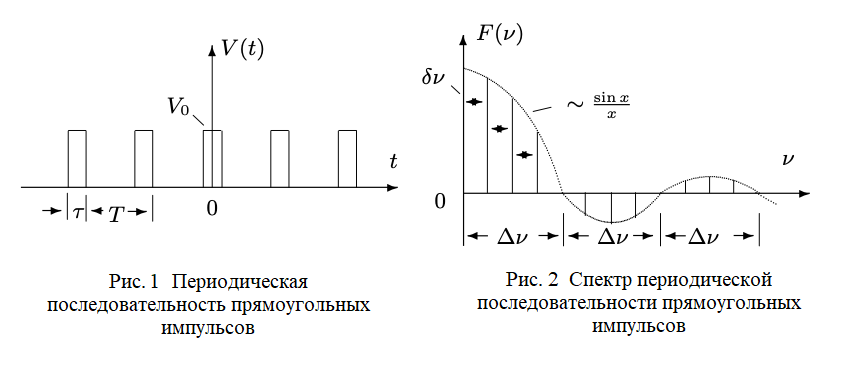
\includegraphics[width=0.7\linewidth]{2.jpg}\\
\end{center}

\subsection{Периодическая последовательность цугов}
\hfill \break Гармонического колебания $V_{0} \cos \left(\omega_{0} t\right)$ с длительностью цуга $\tau$ и периодом повторения $T$ (рис. 3).
\hfill \break
\hfill \break
Функция $f(t)$ снова является чётной относительно $t=0 .$ Амплитуда $n$-й гармоники равна
$$
\begin{array}{c}
A_{n}=a_{n}=\frac{2}{T} \int_{-\tau / 2}^{\tau / 2} V_{0} \cos \left(\omega_{o} t\right) \cdot \cos \left(n \Omega_{1} t\right) d t= \\
=V_{0} \frac{\tau}{T}\left(\frac{\sin \left[\left(\omega_{0}-n \Omega_{1}\right) \frac{\tau}{2}\right]}{\left(\omega_{0}-n \Omega_{1}\right) \frac{\tau}{2}}+\frac{\sin \left[\left(\omega_{0}+n \Omega_{1}\right) \frac{\tau}{2}\right]}{\left(\omega_{0}+n \Omega_{1}\right) \frac{\tau}{2}}\right)
\end{array}
$$
\hfill \break
Такое спектральное распределение F($\omega$) для случая, когда $\frac T\tau$ равно целому числу, представлено на рис. 4. Сравнивая спектр последовательности прямоугольных импульсов и спектр цугов (см. рис. 2 и 4), мы видим, что они практически аналогичны, но их максимумы сдвинуты по частоте на величину $\omega_0$.

\begin{center}
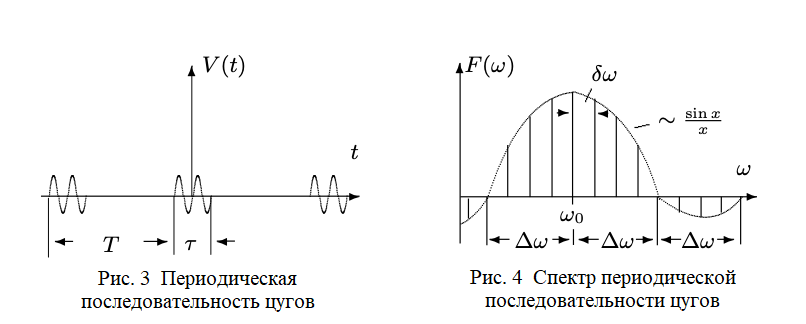
\includegraphics[width=0.7\linewidth]{3.jpg}\\
\end{center}

\subsection{Амплитудно-модулированные колебания.}

\begin{center}
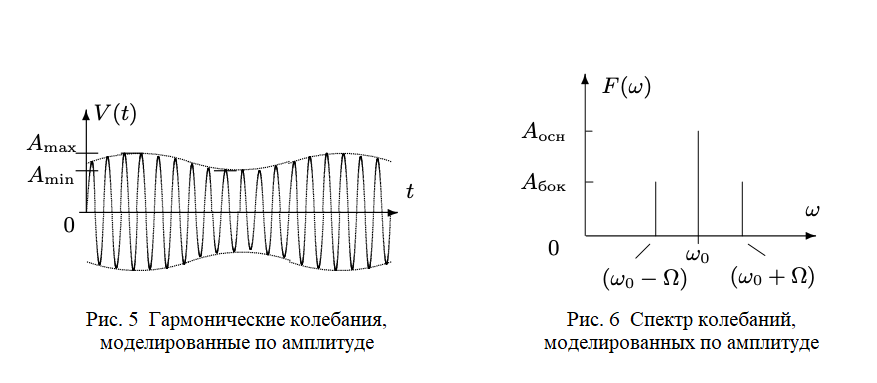
\includegraphics[width=0.7\linewidth]{4.jpg}\\
\end{center}
 Рассмотрим гармонические колебания высокой циклической частоты $\omega_{0},$ амплитуда которых медленно меняется по гармоническому закону с частотой $\Omega\left(\Omega \ll \omega_{0}\right)$ (рис. 5):
$$
f(t)=A_{0}[1+m \cos (\Omega t)] \cos (\omega t)
$$
Коэффициент $m$ называют \textit {глубиной модуляции}. При $m<1$ амплитуда колебаний меняется от минимальной $A_{\min }=A_{0}(1-m)$ до максимальной $A_{\max }=A_{0}(1+m) .$ Глубина модулящии может быть представлена в виде
$$
m=\frac{A_{\max }-A_{\min }}{A_{\max }+A_{\min }}
$$
Простым тригонометрическим преобразованием можно найти спектр амплитудно-модулированных колебаний:
$$
\begin{aligned}
f(t) &=A_{0} \cos \left(\omega_{0} t\right)+A_{0} m \cos (\Omega t) \cos \left(\omega_{0} t\right)=\\
=A_{0} \cos \left(\omega_{0} t\right) &+\frac{A_{0} m}{2} \cos \left(\omega_{0}+\Omega\right) t+\frac{A_{0} m}{2} \cos \left(\omega_{0}-\Omega\right) t
\end{aligned}
$$
\hfill \break
Спектр $F(\omega)$ таких колебаний содержит три составляющие (рис. 6$)$. Основная компонента представляет собой исходное немодулированное колебание с несущей частотой $\omega_{0}$ и амплитудой $A_{\text{ocн}}=A_{0}-$ первое слагаемое в правой части; боковые компоненты спектра соответствуют гармоническим колебаниям с частотами $\left(\omega_{0}+\Omega\right)$ и $\left(\omega_{0}-\Omega\right)-$ второе и третье слагаемые. Амплитуды этих двух колебаний одинаковы и составляют $m / 2$ от амплитуды немодулированного колебания: $A_{\text {бок }}=A_{0} m / 2$

\section{Экспериментальная установка}
\hfill \break
Схема установки представлена на рисунке:

\begin{center}
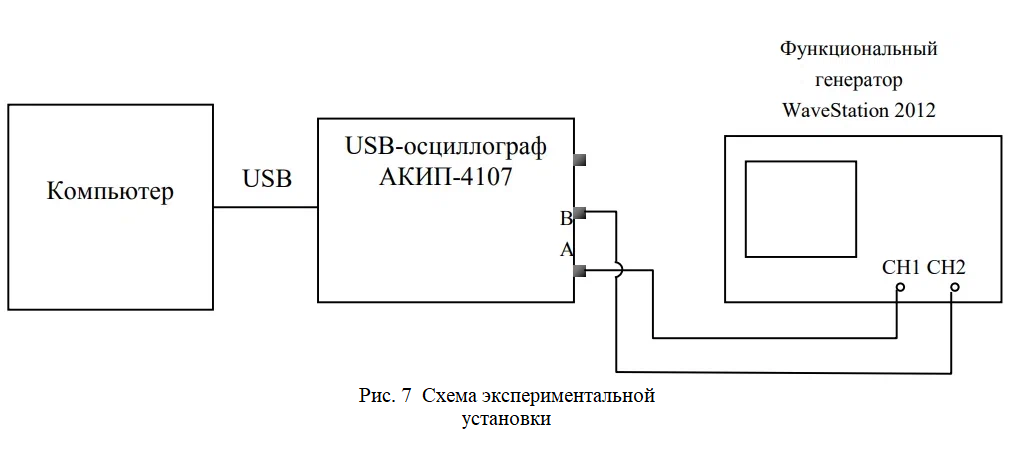
\includegraphics[width=0.8\linewidth]{5.png}\\
\end{center}

\hfill \break
Функциональный генератор WaveStation 2012 позволяет сформировать два различных электрических сигнала, которые выводятся на два независимых канала – CH1 и CH2. Сигнал с канала CH1 подается на вход А, а
сигнал с канала CH2 – на вход В USB-осциллографа. Затем эти сигналы подаются на вход компьютера через USB-соединение. При работе USB-осциллографа в режиме осциллографа на экране компьютера можно наблюдать каждый из сигналов в отдельности, а также их произведение. В режиме спектроанализатора можно наблюдать спектры этих сигналов.

\section{Ход работы}

\hfill \break Соберем схему и подготовим приборы к работе, следуя техническому описанию.

\subsection{А. Исследование спектра периодической последовательности прямоугольных импульсов}

\hfill \break На генераторе установим частоту повторения импульсов $f_{\text {повт}}=1 }$ кГц и длительность импульса $\tau=100$ мкс. Проанализируем, как изменится наблюдаемый спектр при увеличении $\tau$ до 200 мкс и неизменной частоте повторения $f_{\text {повт}}$; при увеличении частоты повторения до 2 кГц и неизменной длительности импульса $\tau$:

\hfill \break \begin{center}
\begin{tabular}{cc}
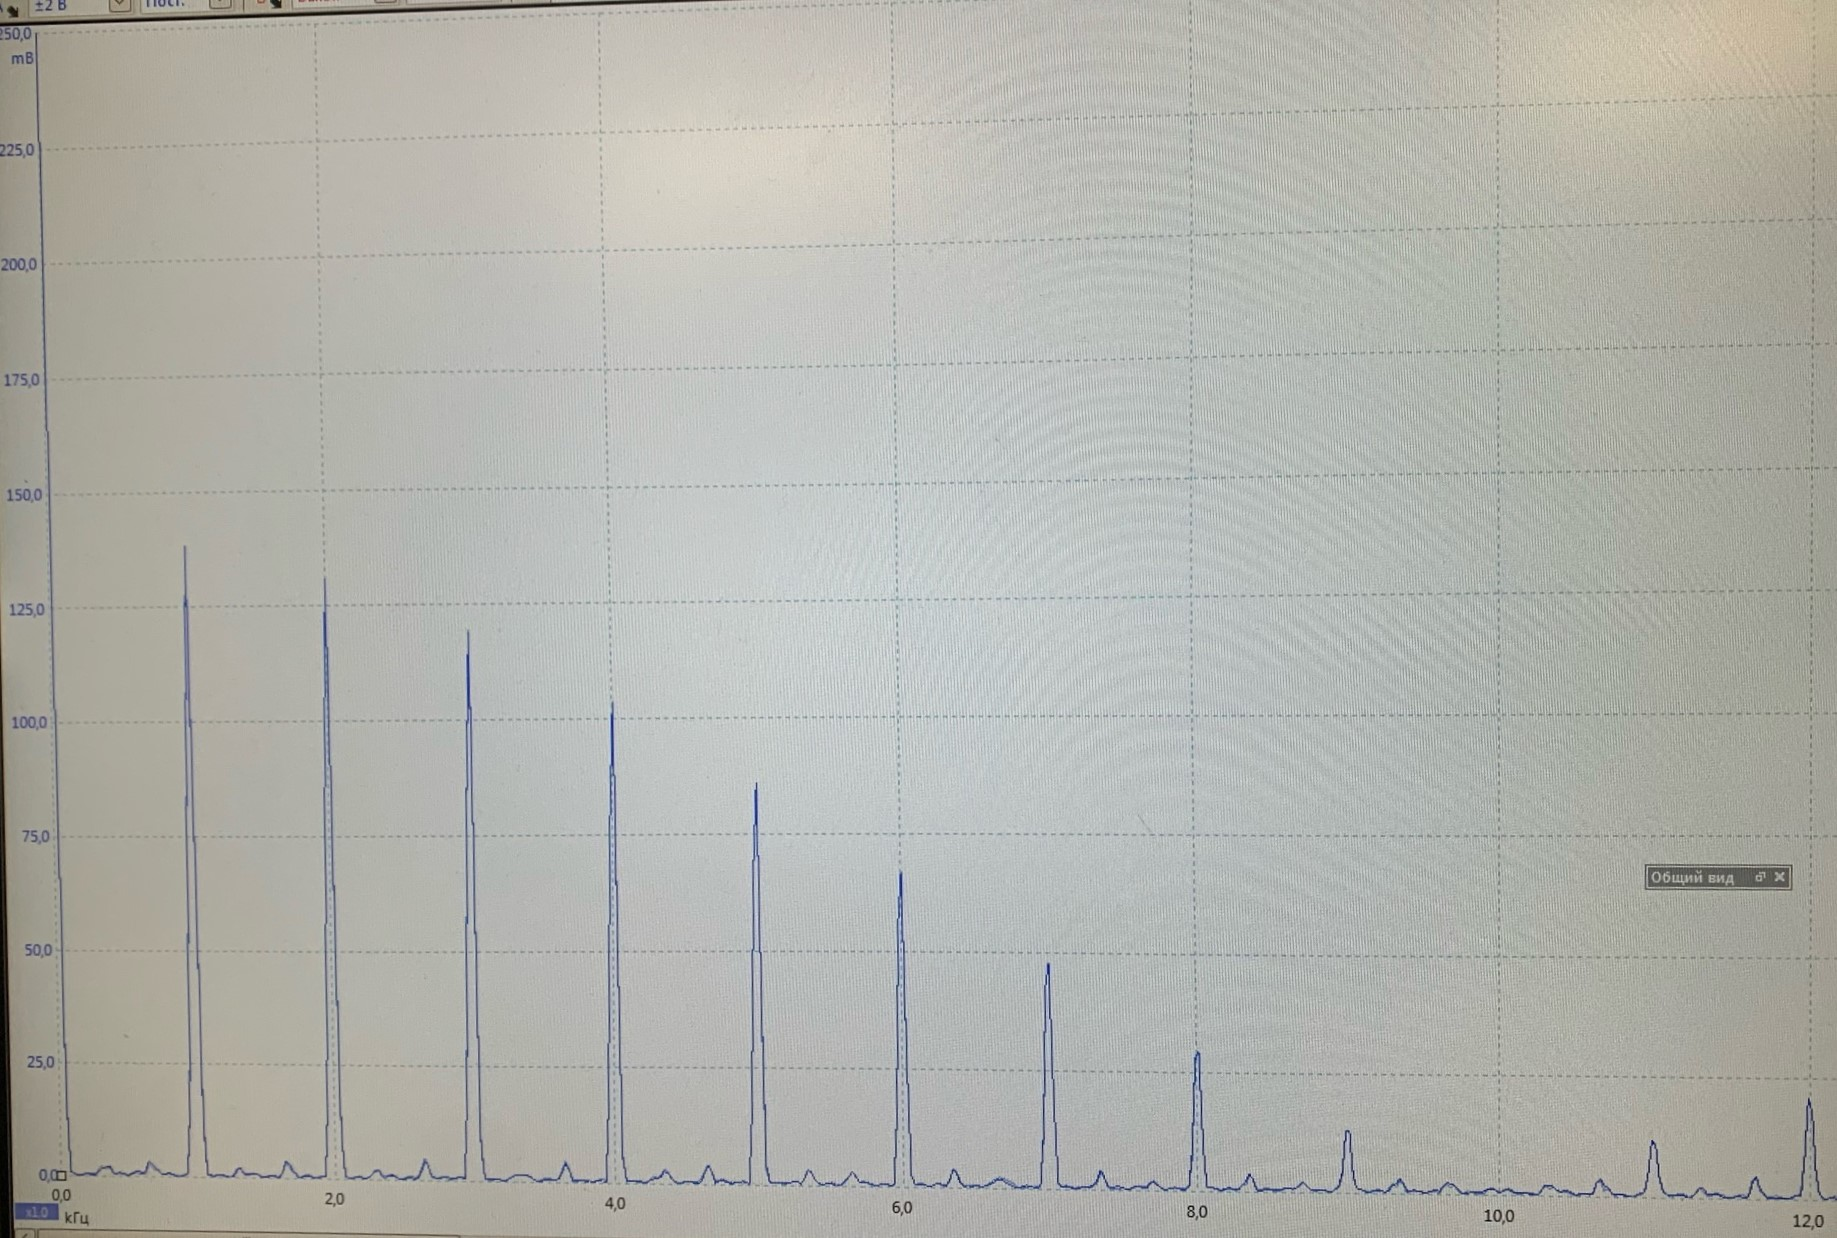
\includegraphics[width=0.45\textwidth]{6.jpg}&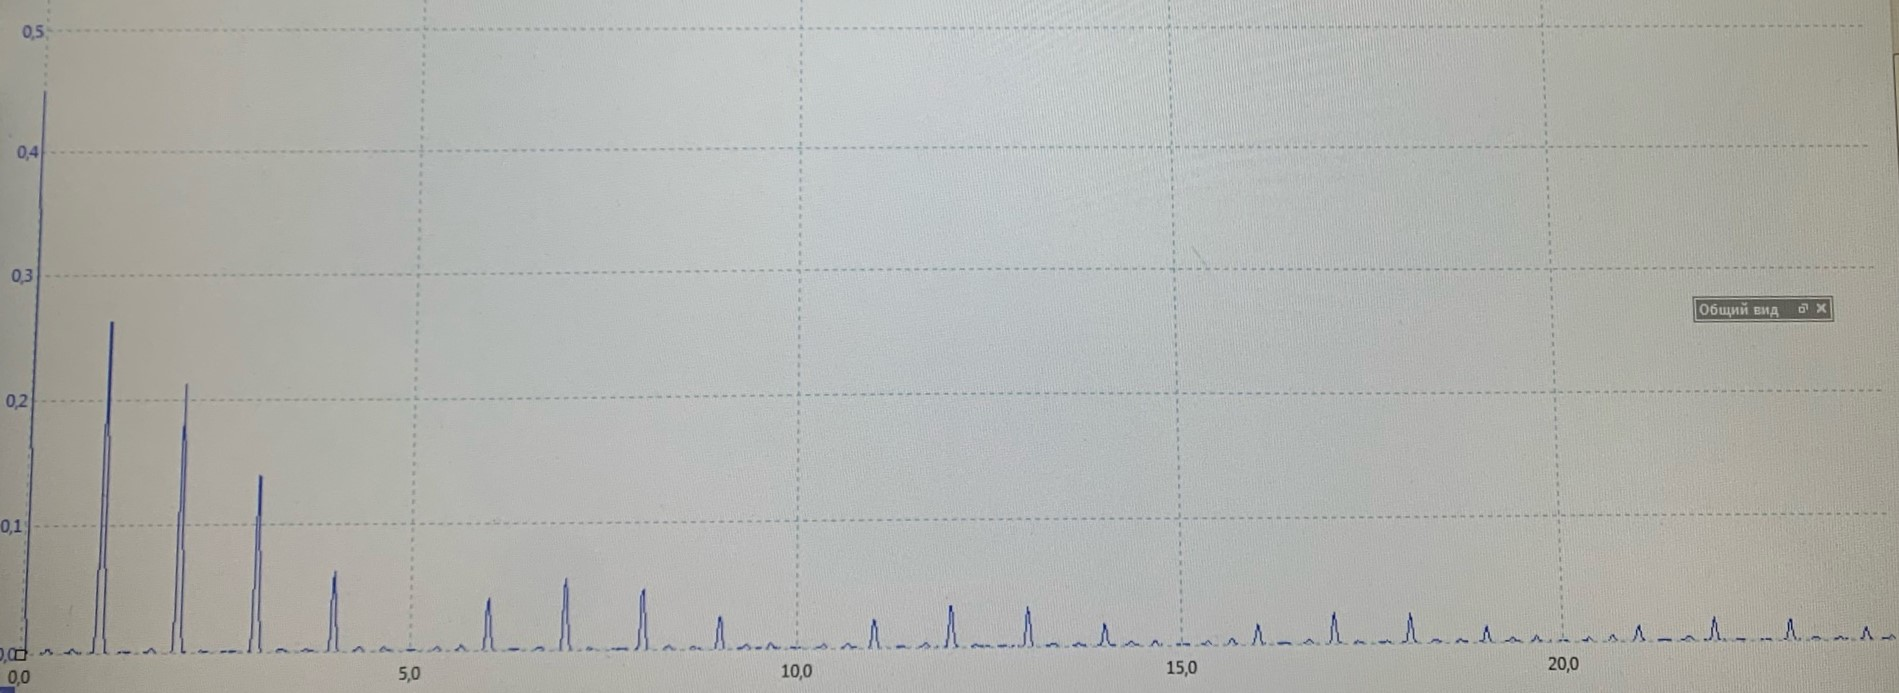
\includegraphics[width=0.45\textwidth]{7.jpg}\\
$f_{\text{повт}} = 1$ кГц, $\tau = 100$ мкс&$f_{\text{повт}} = 1$ кГц, $\tau = 200$ мкс\\
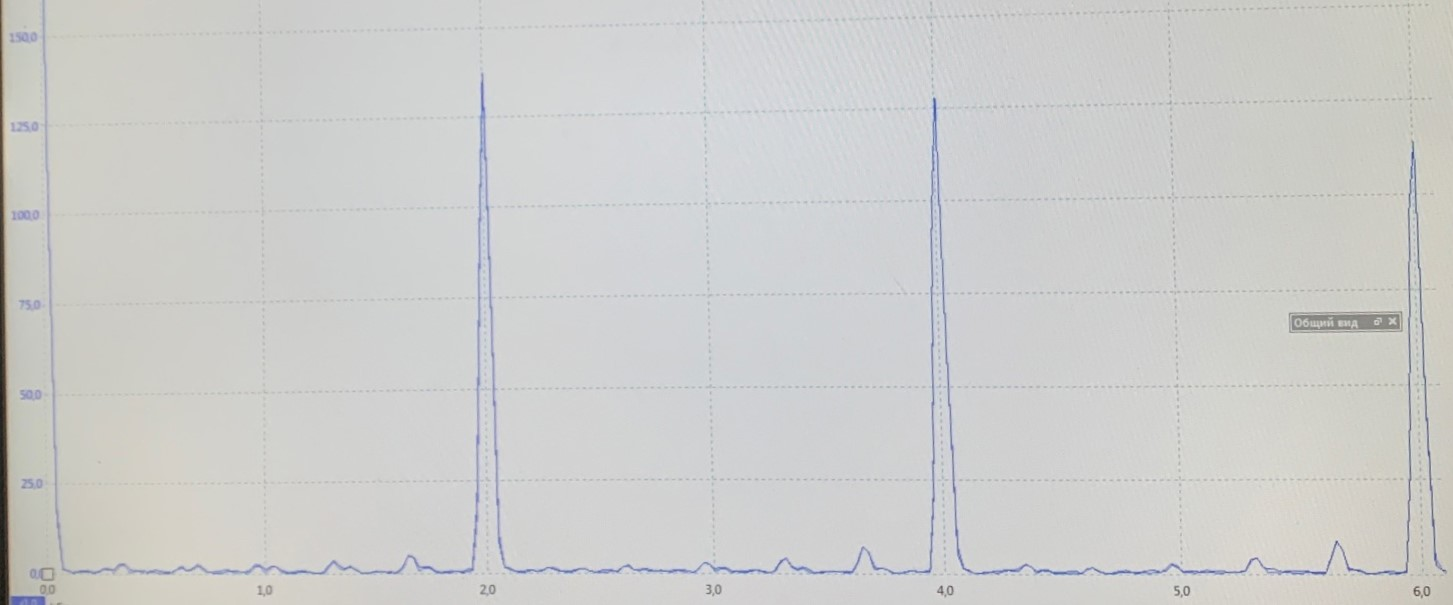
\includegraphics[width=0.45\textwidth]{8.jpg}\\
$f_{\text{повт}} = 2$ кГц, $\tau = 100$ мкс\\
\end{tabular}
\end{center}

\hfill \break Из полученных изображений видно, что при увеличении $\tau$ вдвое $\Delta \nu$ уменьшается в два раза, а при увеличении $f_\text{повт}$ увеличивается расстояние между пиками $\delta \nu$. Проведем измерения зависимости ширины спектра $\Delta \nu$ от длительности импульса $\tau$ при увеличении $\tau$ от 40 до 200 мкс и на основе полученных данных построим график зависимости $\Delta \nu$(1/$\tau$).\\

\hfill \break \begin{center}
\begin{tabular}{|c|c|c|}\hline
$\tau\text{, мкс}$&$1/\tau, $ мкс^{-1}$ \cdot 10^2 $$&$\Delta\nu, $ кГц$ \cdot 10^{-1} \\\hline
$200$&$0.50$&$0.50$\\\hline
$180$&$0.56$&$0.55$\\\hline
$160$&$0.63$&$0.65$\\\hline
$140$&$0.71$&$0.70$\\\hline
$120$&$0.83$&$0.80$\\\hline
$100$&$1.00$&$1.00$\\\hline
$80$&$1.25$&$1.20$\\\hline
$60$&$1.67$&$1.70$\\\hline
$40$&$2.50$&$2.50$\\\hline
\end{tabular}\\
\hfill \break \textbf {Таблица 1.} Исследование зависимости $\Delta \nu$(1/$\tau$)~\\
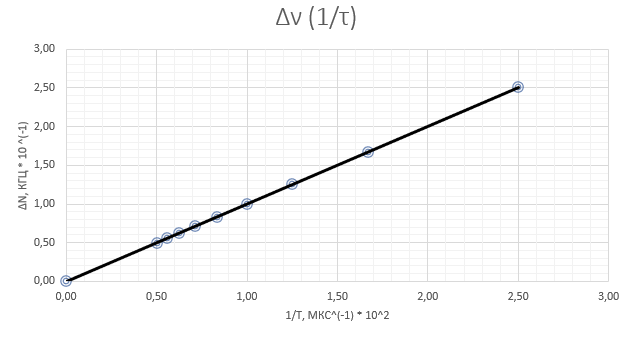
\includegraphics[width=0.95\textwidth]{9.png}\\
График зависимости $\Delta \nu$(1/$\tau$)\\
\end{center}

\hfill \break Коэффициент наклона полученного графика $k$ = 1.0046 = $\Delta \nu \cdot \tau$, что подтверждает соотношение неопределенностей. Теперь зафискируем $f_\text{повт}=1$ кГц и $\tau=50$ мкс. Для этих параметров посмотрим амплитуду $n-$й гармоники $a_{n}$ и частоту $f_{n}$. Амплитуды сравним с рассчитанными теоретически.

\begin{center}
\begin{tabular}{|c|c|c|c|c|c|}
\hline
$n$ гармоники & 1 & 2 & 3 & 4 & 5 \\\hline
$f$, кГц & 29,4 & 49,4 & 69,6 & 89,8 & 110 \\\hline
$a_n$, мВ & 13,9 & 8,9 & 7,5 & 5,2 & 4,4 \\\hline
$a_{n, \text{теория}}$, мВ & 11,6 & 10,3 & 8,4 & 6,1 & 3,6 \\\hline
\end{tabular}

\hfill \break \textbf{Таблица 2.} Исследование амплитуд и частот гармоник. 
\end{center}

\hfill \break Видим, что амплитуды довольно неплохо сходятся с теорией, что подтверждает приведенную выше формулу.

\subsection{Б. Исследование спектра периодической последовательности цугов гармонических колебаний}

\begin{center}
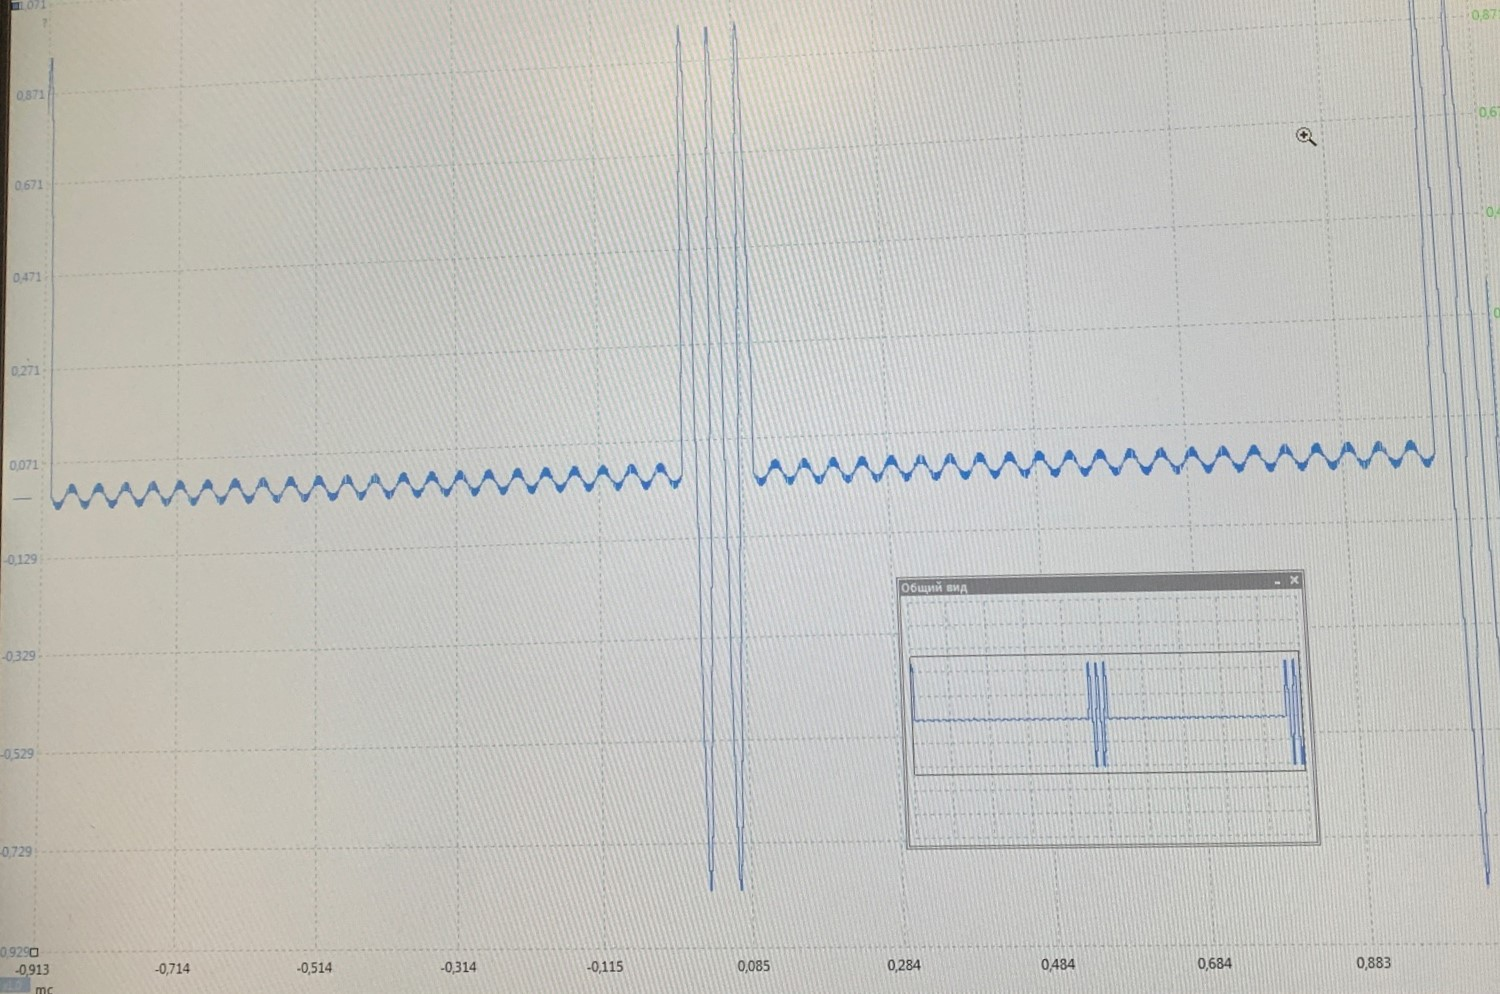
\includegraphics[width=0.6\linewidth]{20.jpg}\\
Периодическая последовательность цугов\\
\end{center}

\hfill \break В этой части исследуется зависимость расстояния между ближайшими спектральными компонентами от частоты повторения цугов. Установим частоту несущей $\nu_{0}=$ 25 кГц и проанализируем, как изменяется вид спектра цугов:
\hfill \break \hfill \break а) при частоте повторения импульсов $f_\text{повт}=$ 1 кГц и длительности импульса $\tau$, изменяющейся от 100 мкс до 200 мкс, видно, что увеличивается амплитуда и ширина пиков становится меньше в два раза:

\hfill \break \begin{center}
\begin{tabular}{cc}
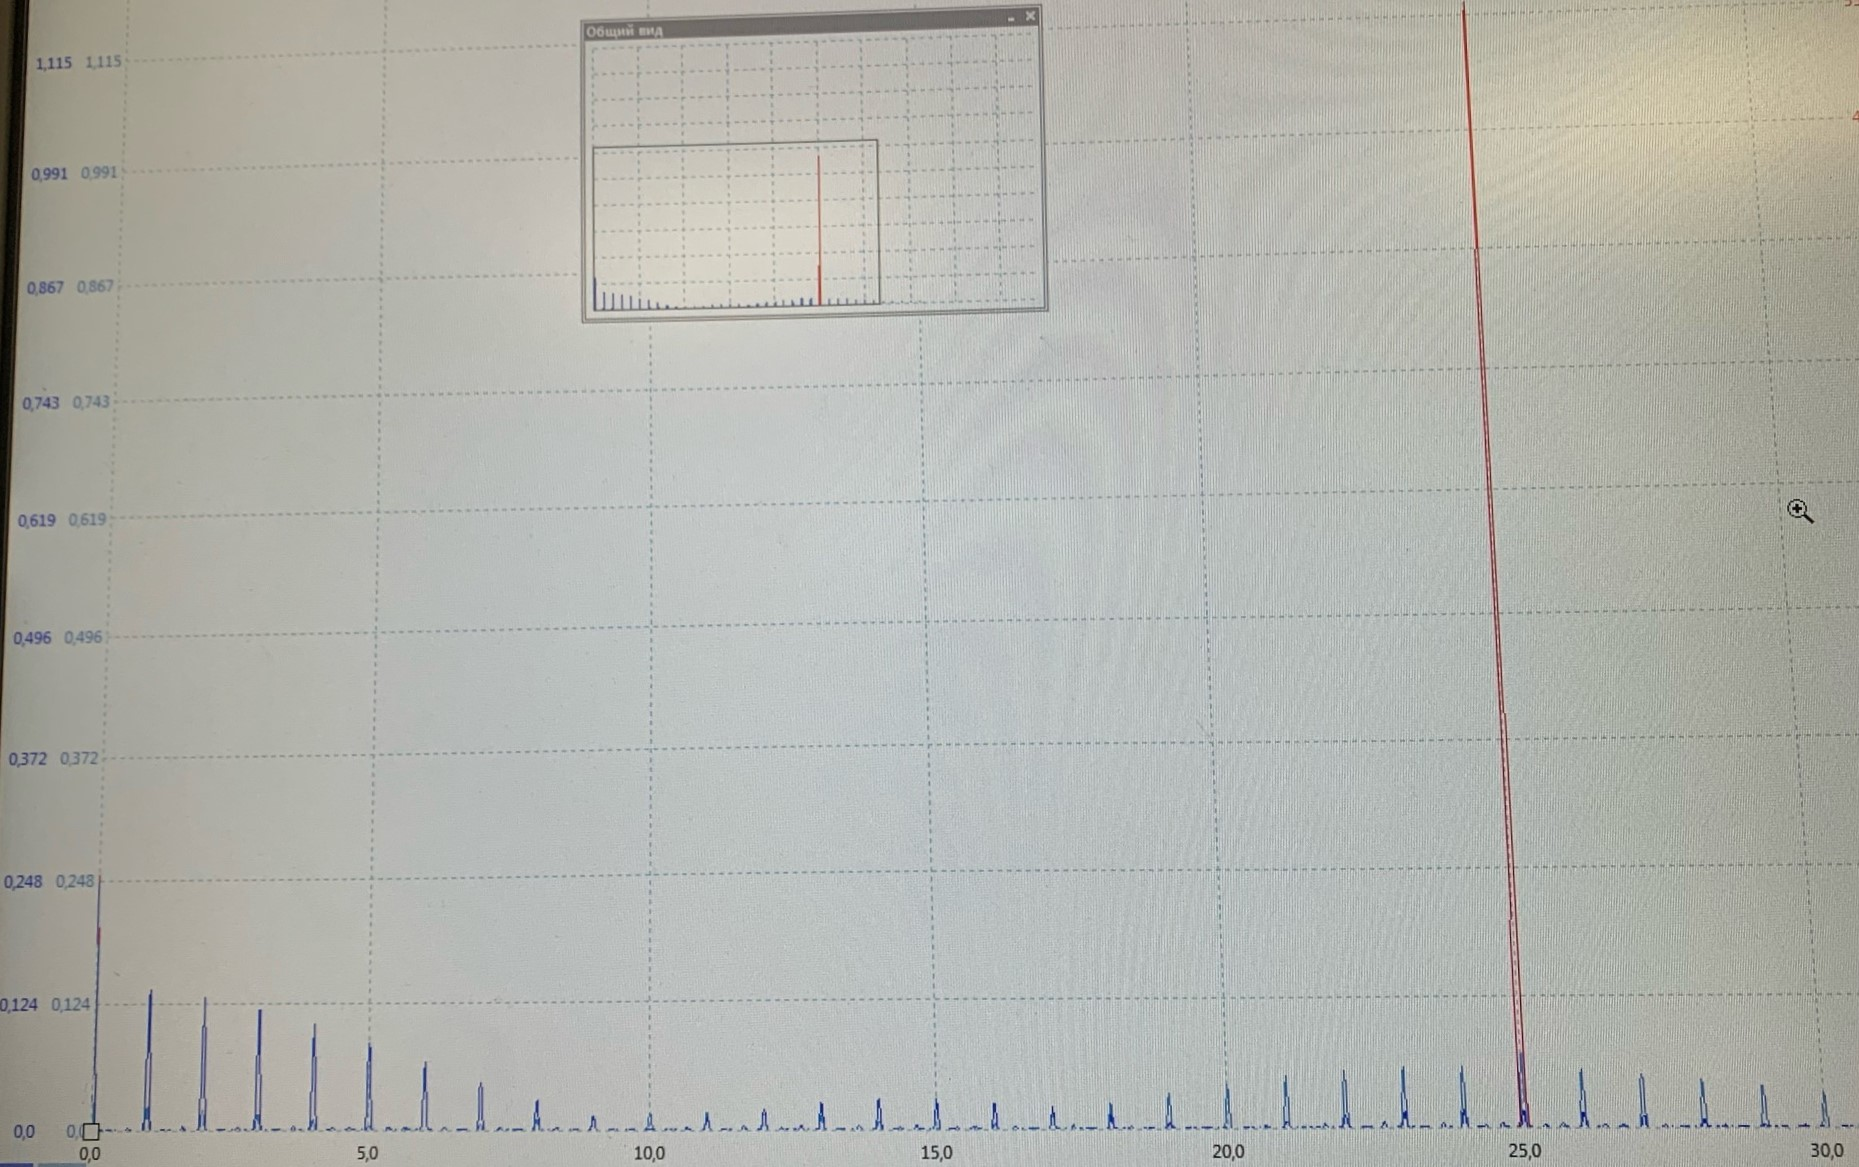
\includegraphics[width=0.45\textwidth]{9.jpg}&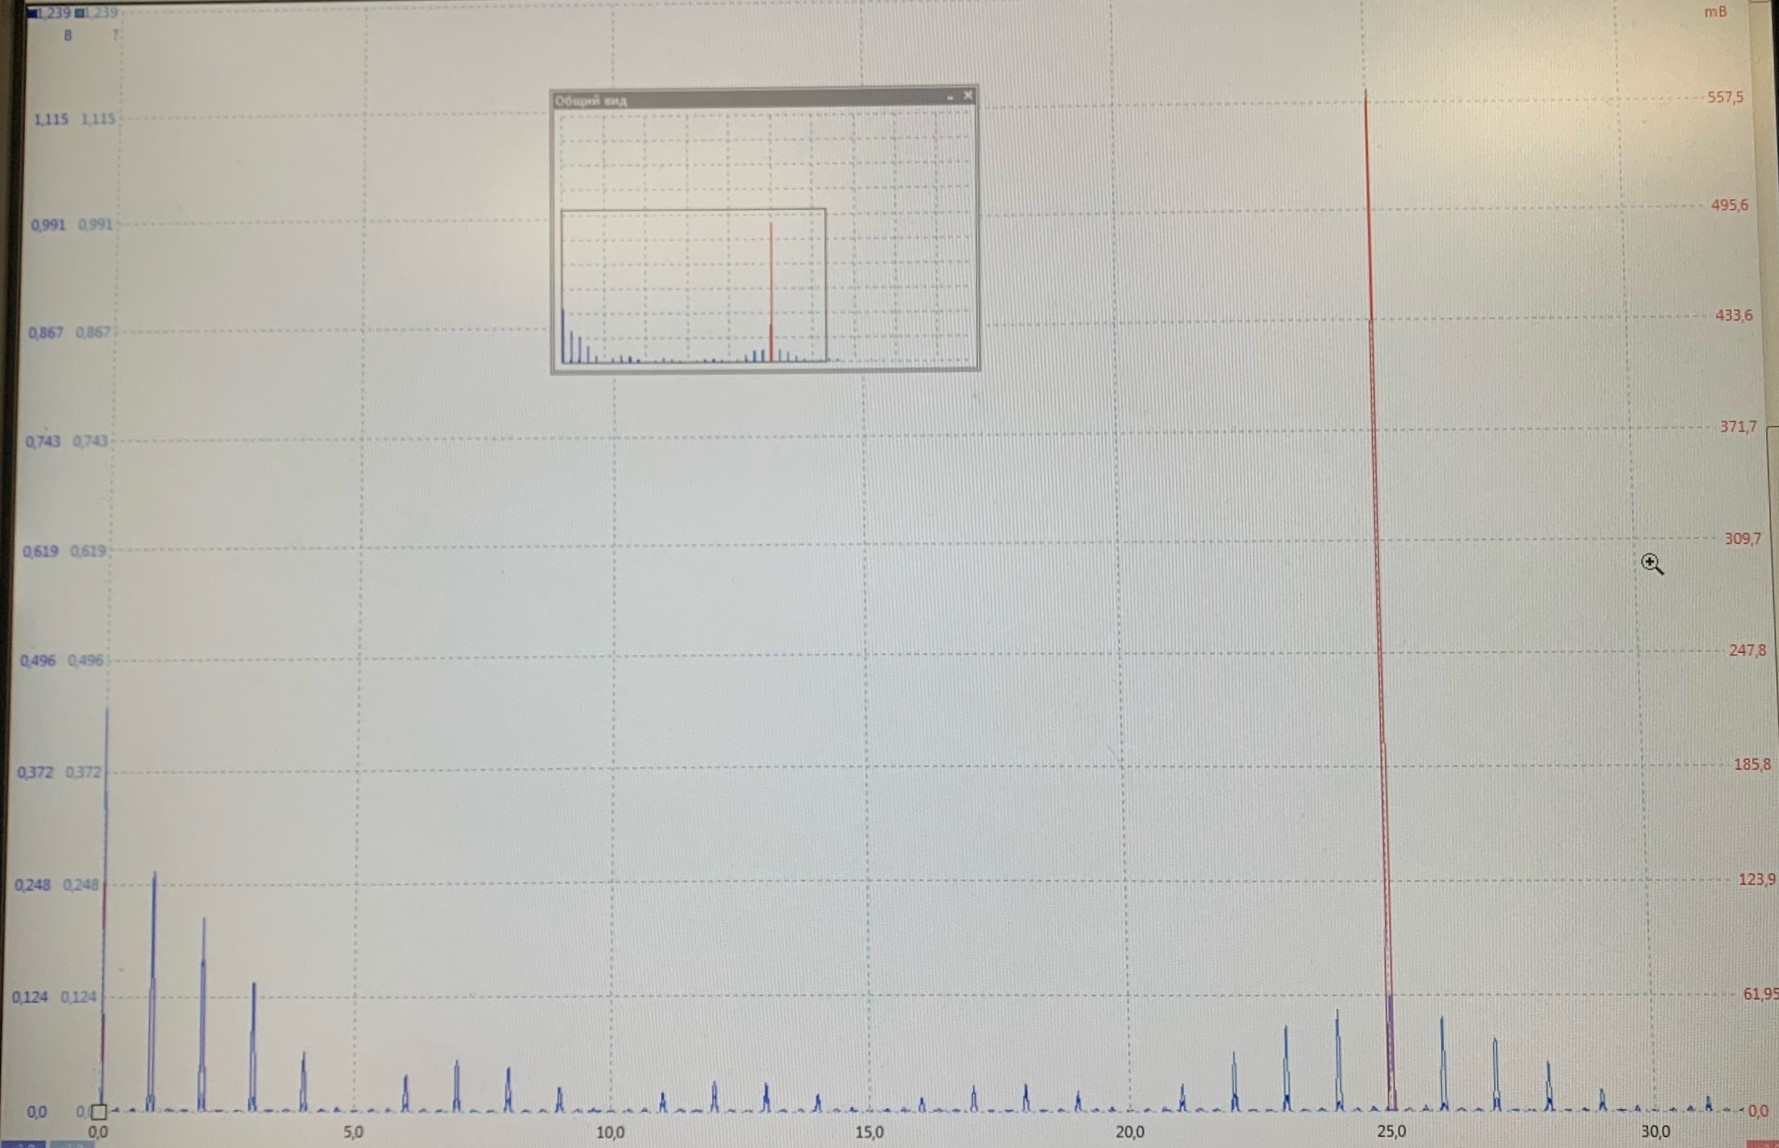
\includegraphics[width=0.45\textwidth]{10.jpg}\\
$\tau=$ 100 мкс&$\tau=$ 200 мкс\\
\end{tabular}
\end{center}

\hfill \break \hfill \break б) при длительности импульса $\tau$ = 100 мкс и изменении частоты несущей $\nu_{0}$ = 10, 25, 40 кГц смещается пик без изменения расстояния между спектральными компонентами:

\hfill \break \begin{center}
\begin{tabular}{cc}
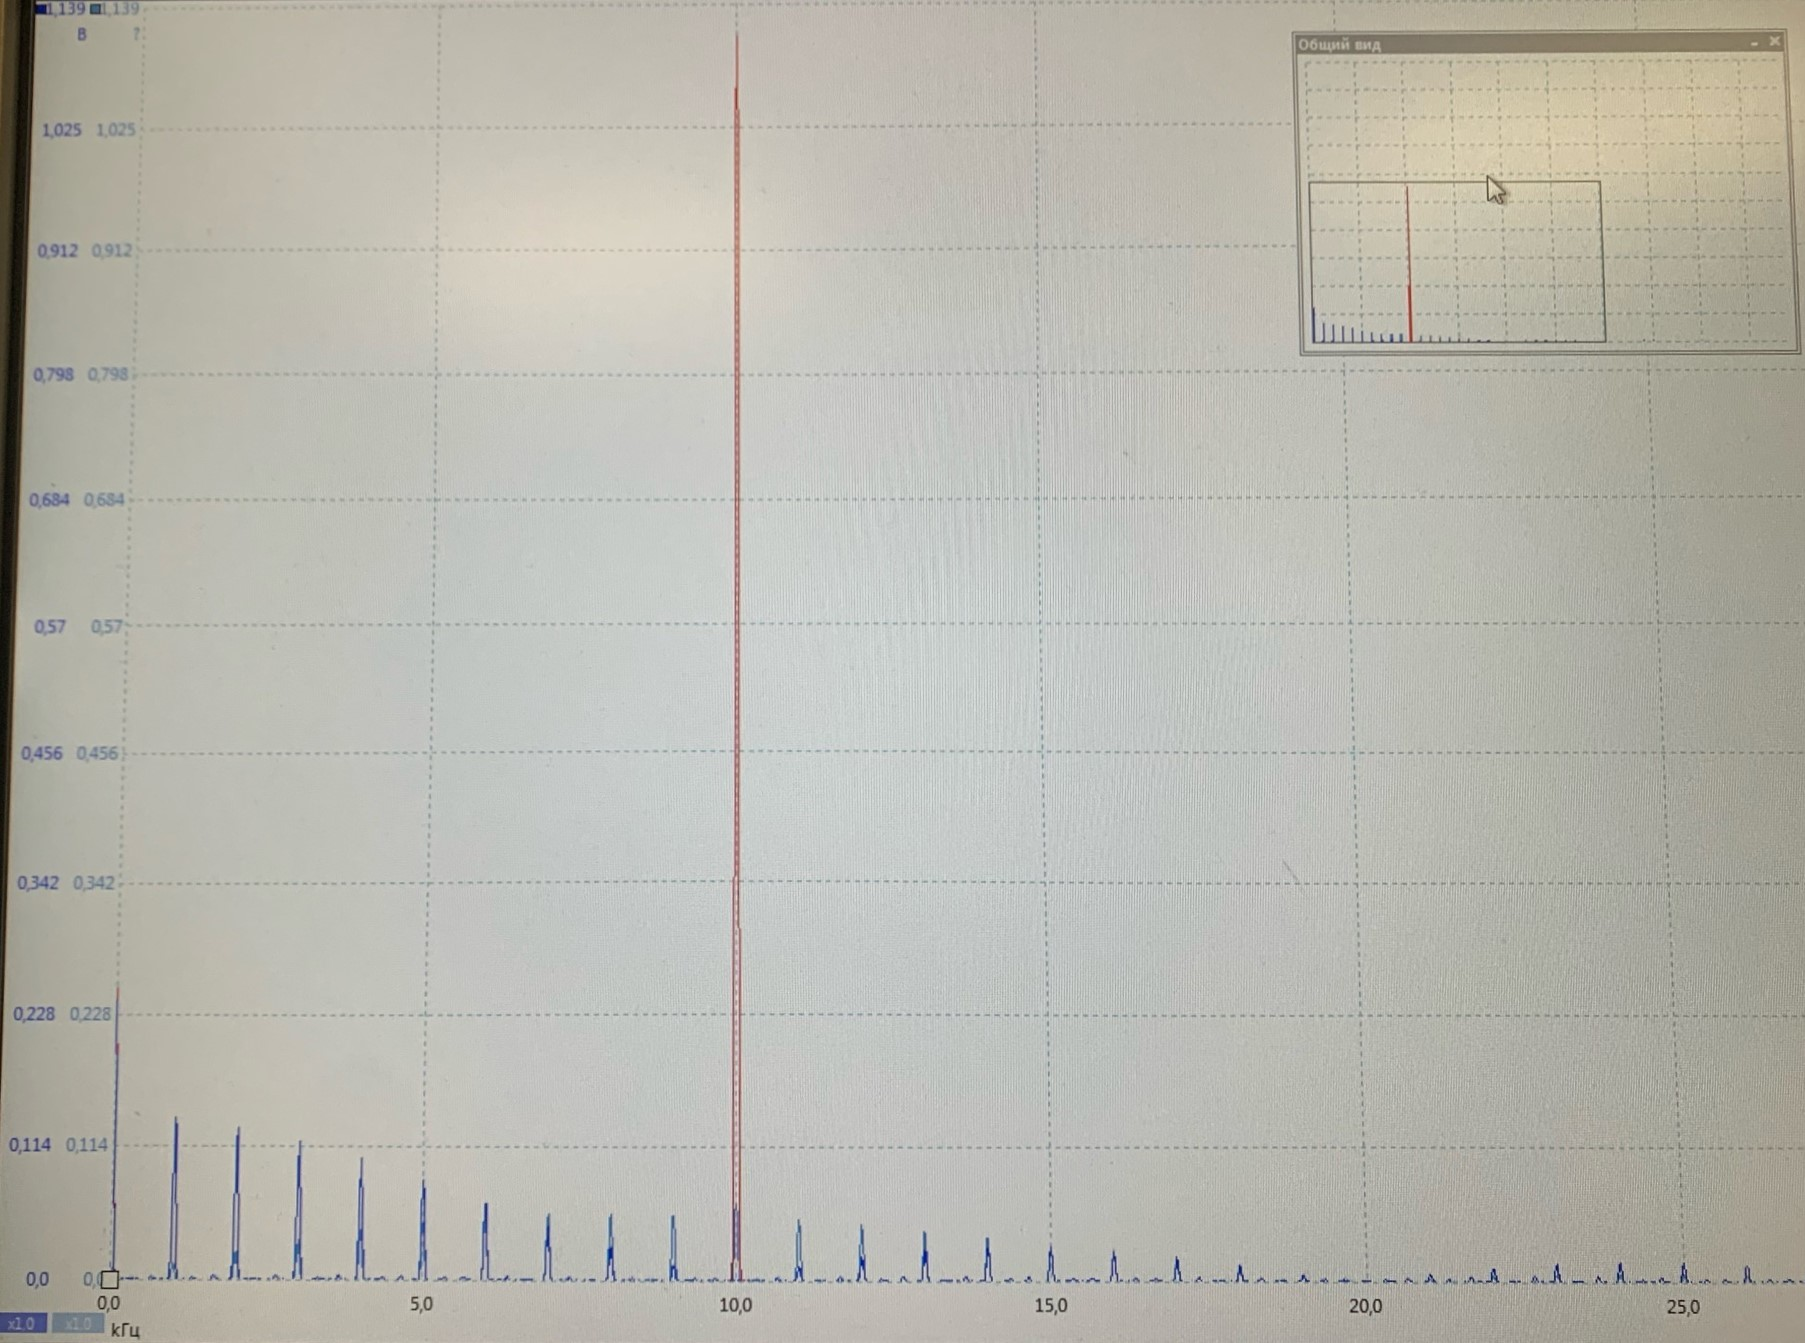
\includegraphics[width=0.45\textwidth]{11.jpg}&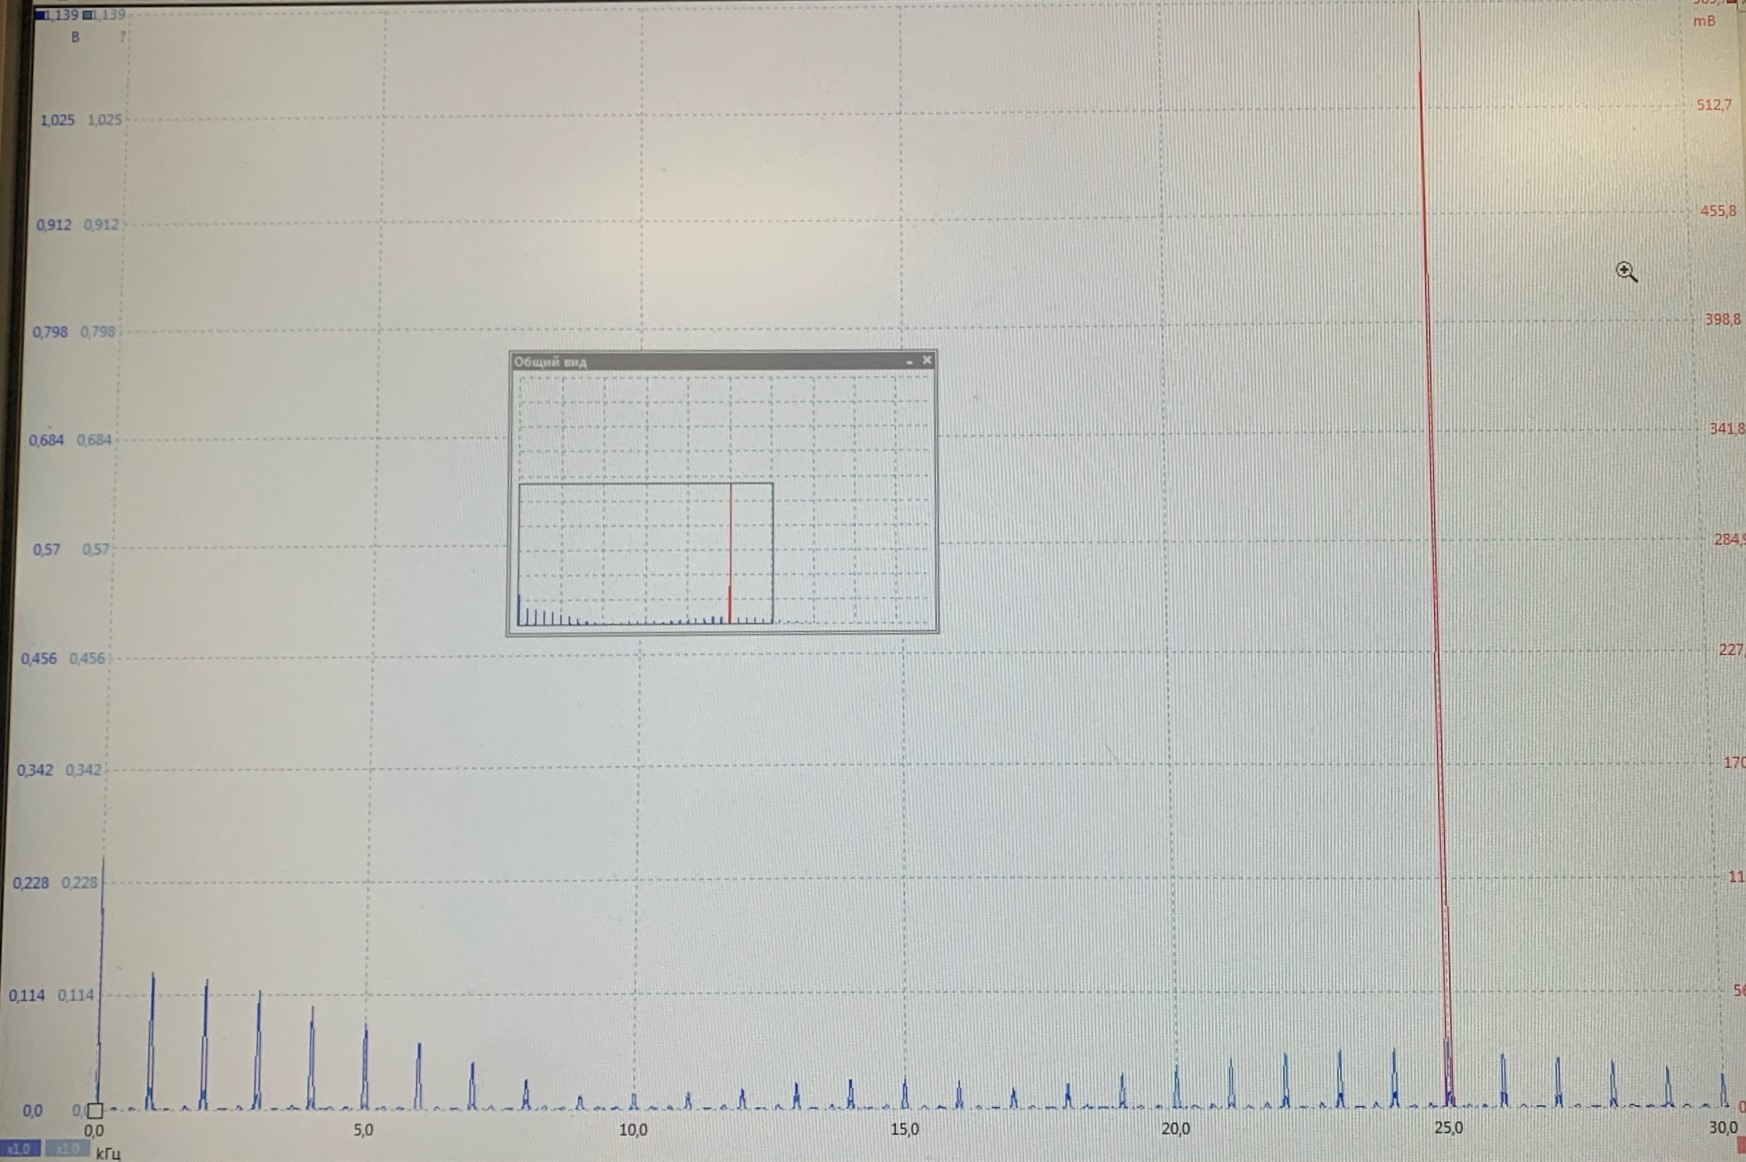
\includegraphics[width=0.45\textwidth]{12.jpg}\\
$\nu_{0}$ = 10 кГц&$\nu_{0}$ = 25 кГц\\
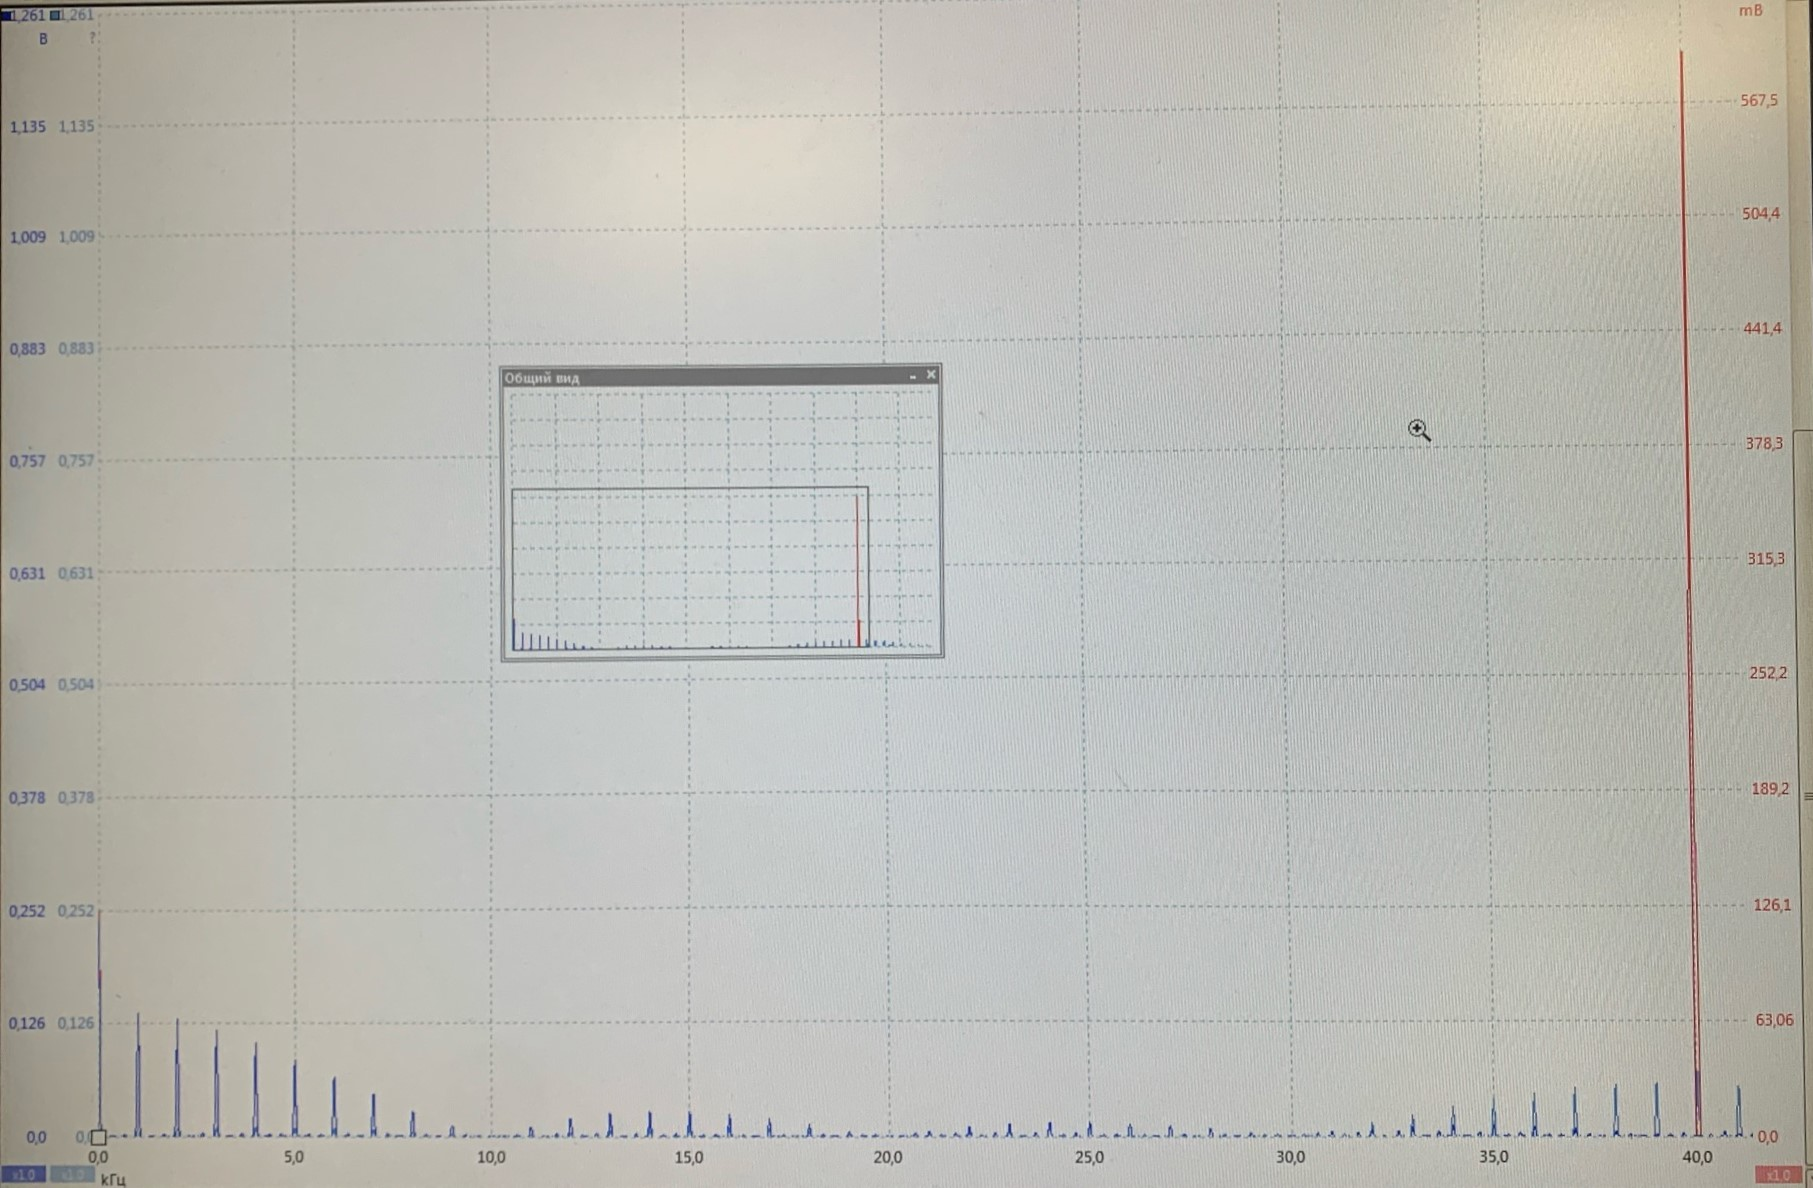
\includegraphics[width=0.45\textwidth]{13.jpg}\\
$\nu_{0}$ = 40 кГц\\
\end{tabular}
\end{center}

\hfill \break Теперь зафиксируем частоту несущей $\nu_{0}=$ 30 кГц и длительность импульса $\tau = $ 100 мкс. Для разных частот повторения импульсов ($f_\text{повт}=$ 0.5, 1, 2, 4, 5 кГц) будем определять расстояние между соседними спектральными компонентами $\delta\nu$:

\hfill \break \begin{center}
\begin{tabular}{cc}
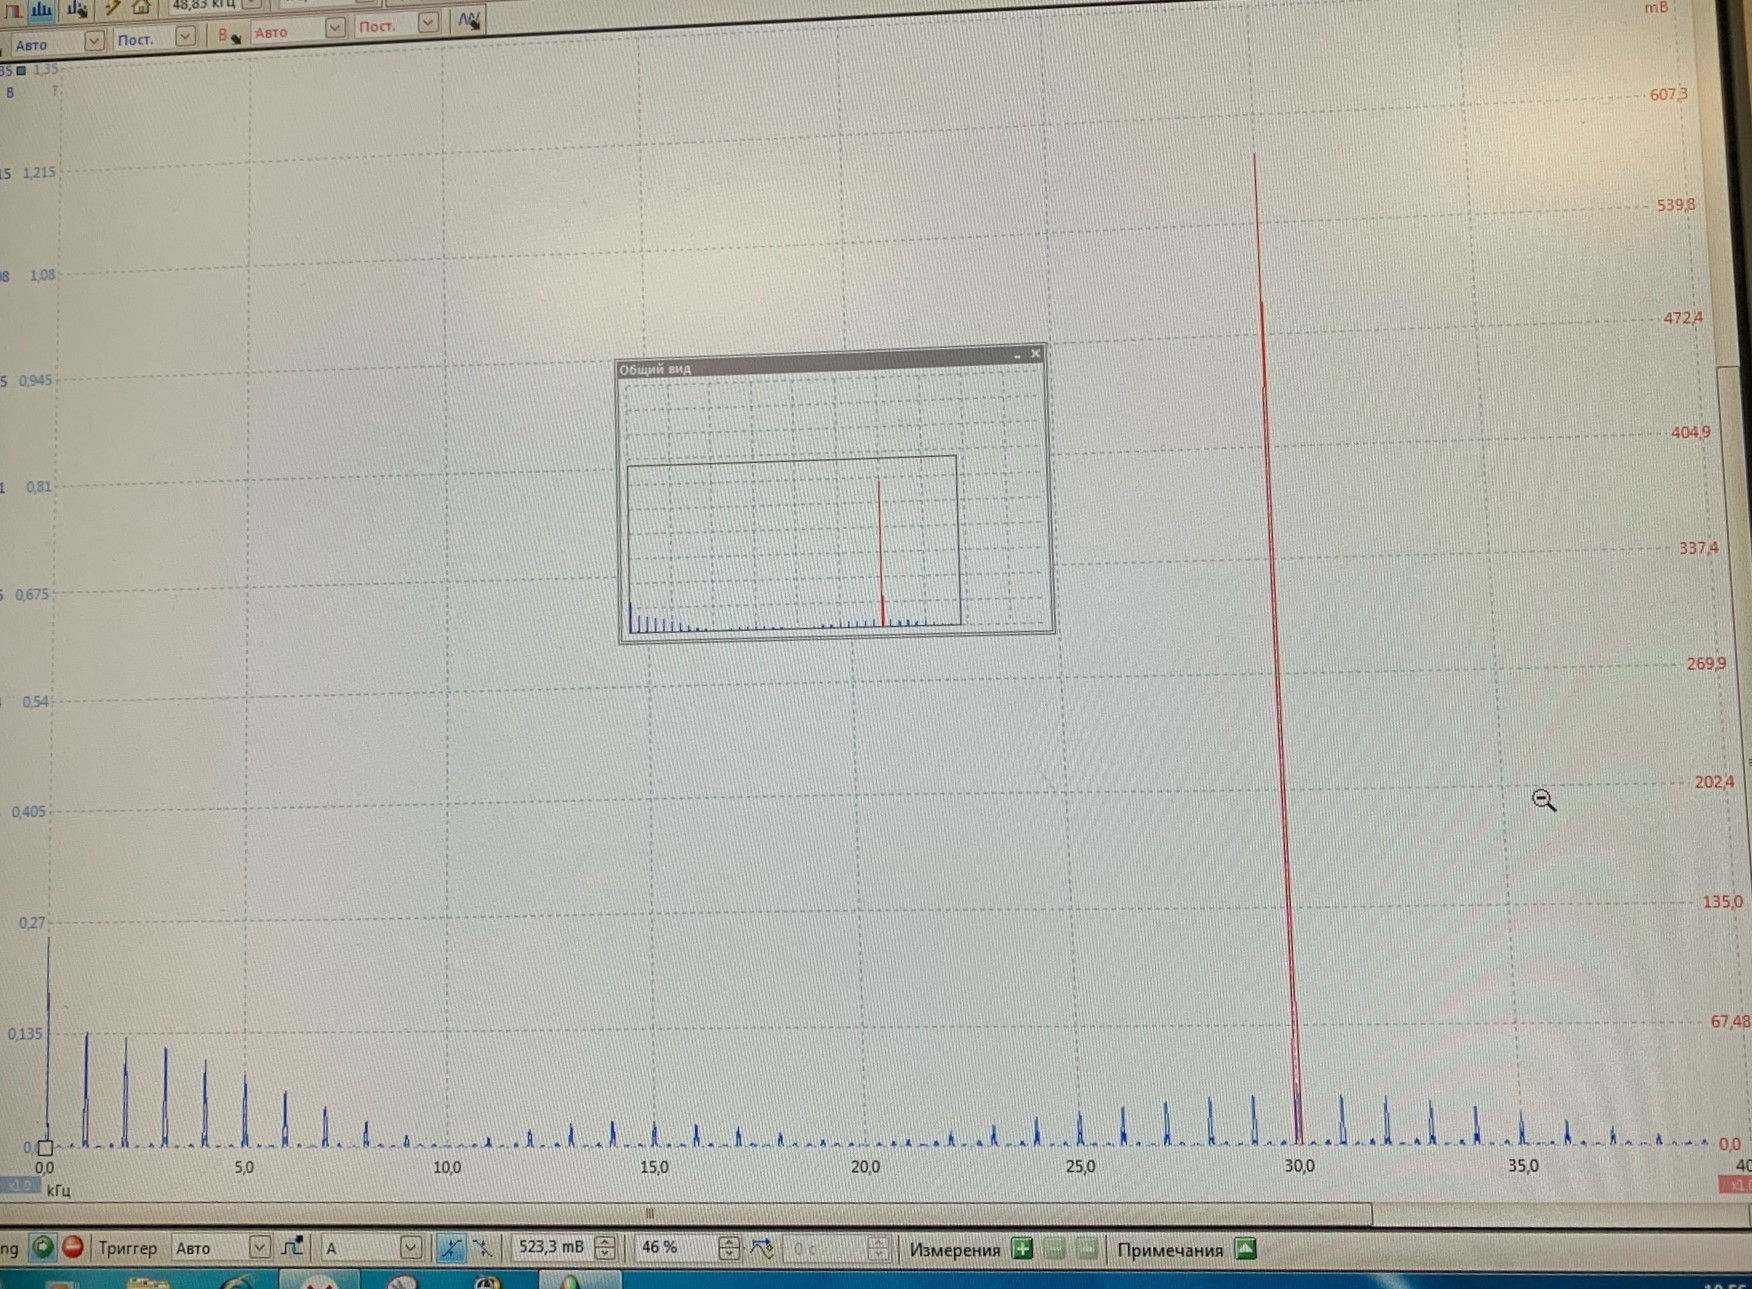
\includegraphics[width=0.45\textwidth]{14.jpg}&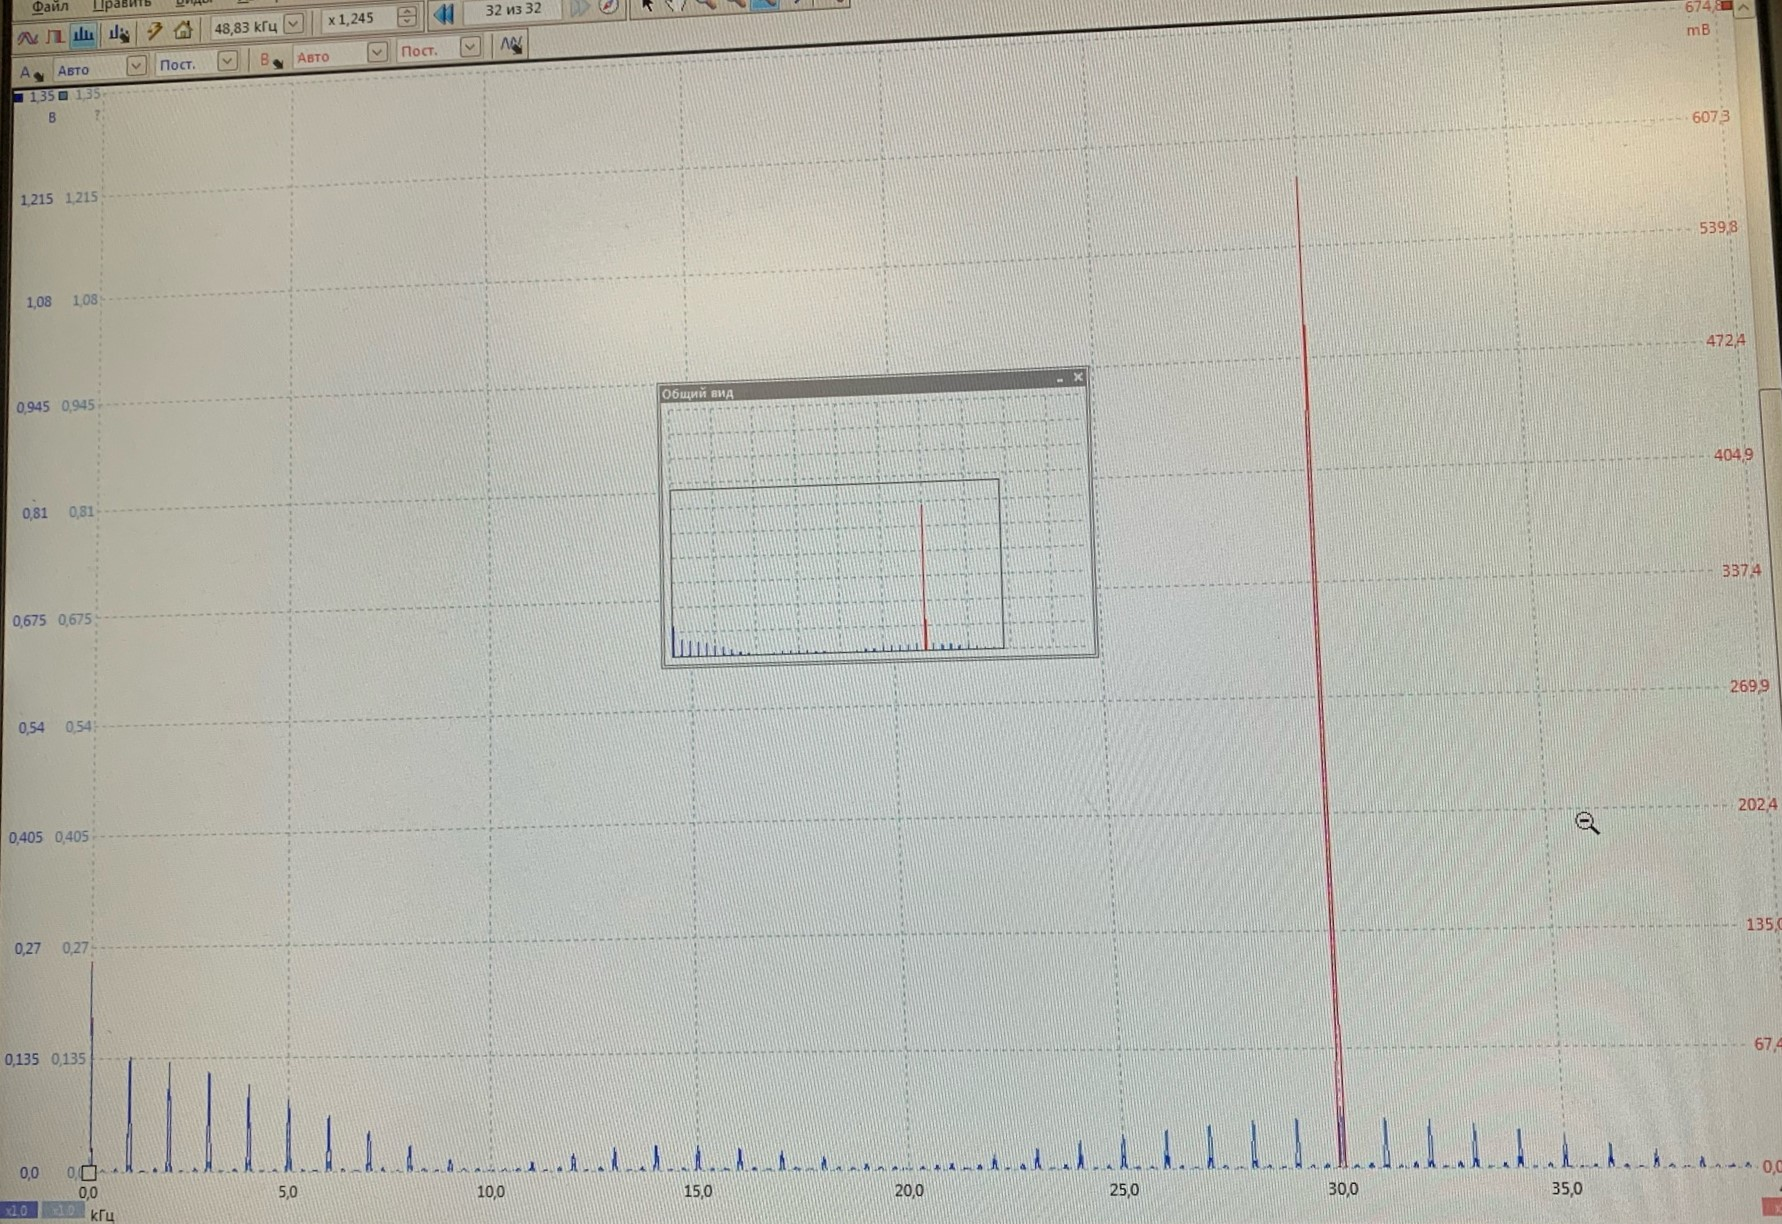
\includegraphics[width=0.45\textwidth]{15.jpg}\\
$f_\text{повт}=$ 0.5 кГц&$f_\text{повт}=$ 1 кГц\\
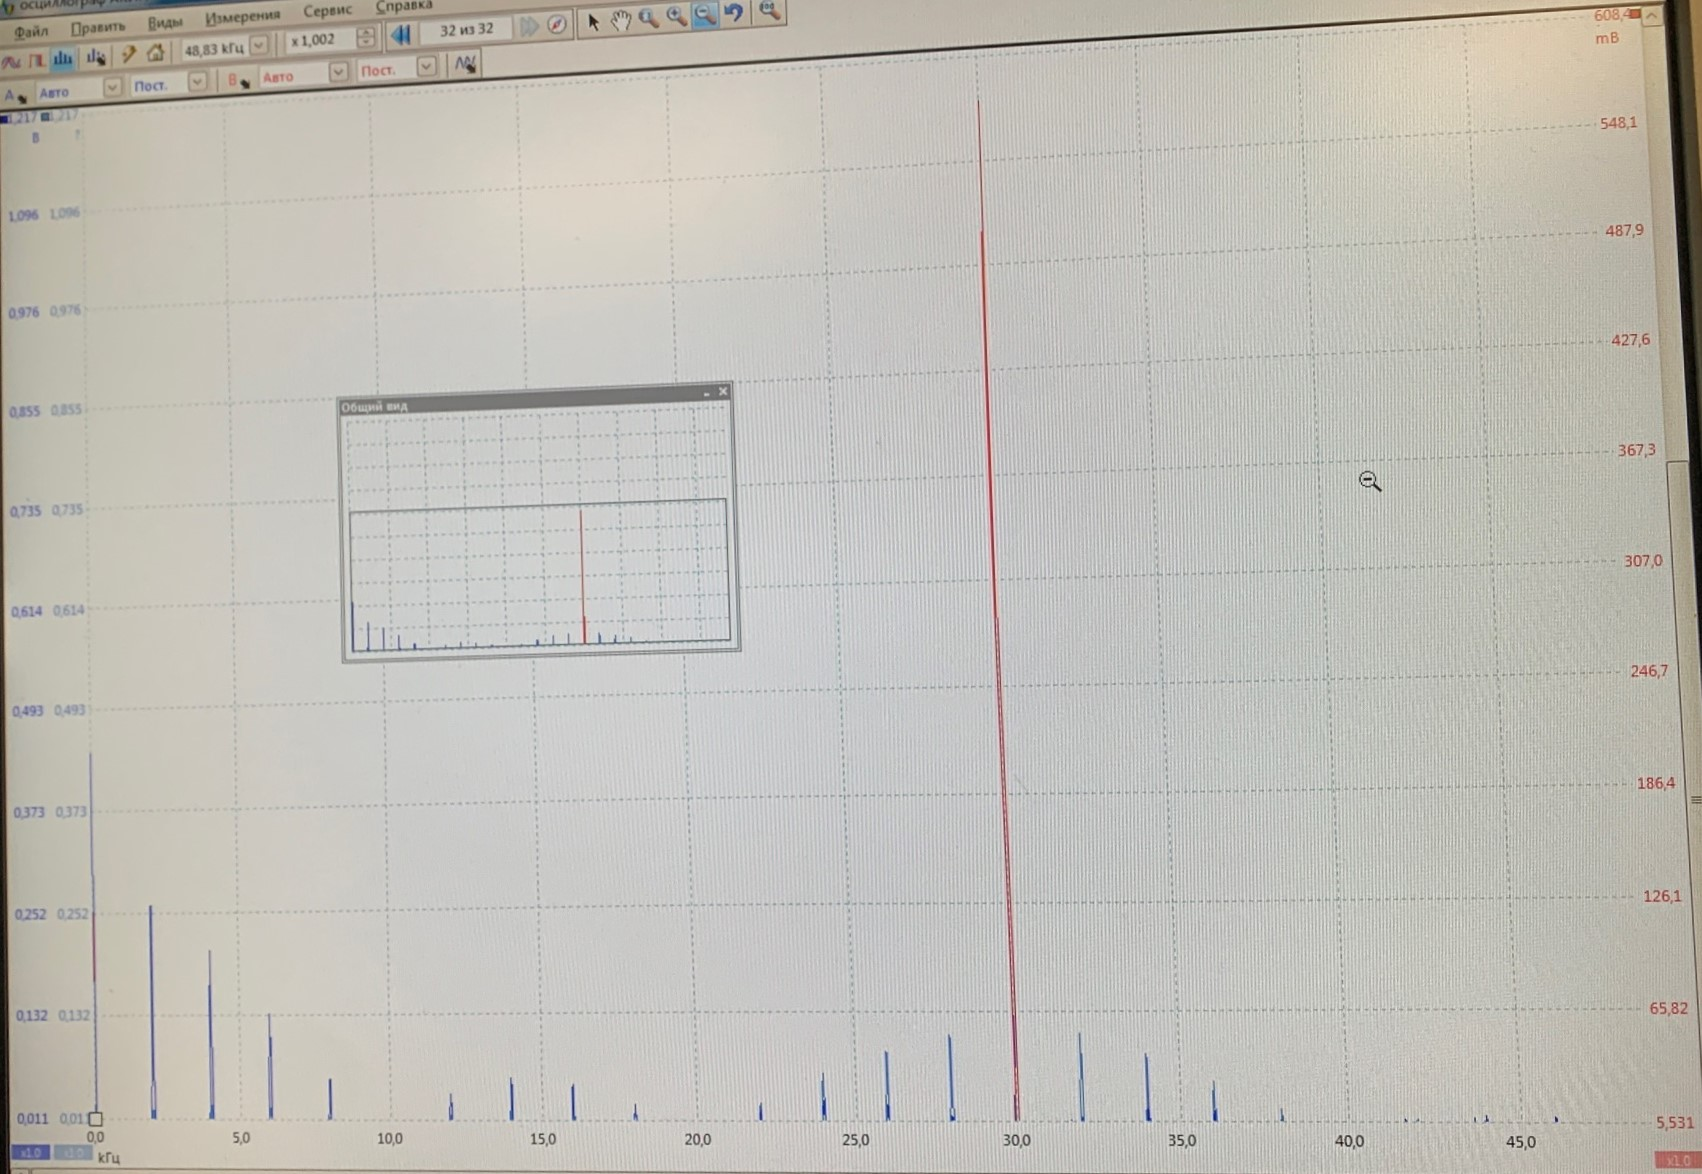
\includegraphics[width=0.45\textwidth]{16.jpg}&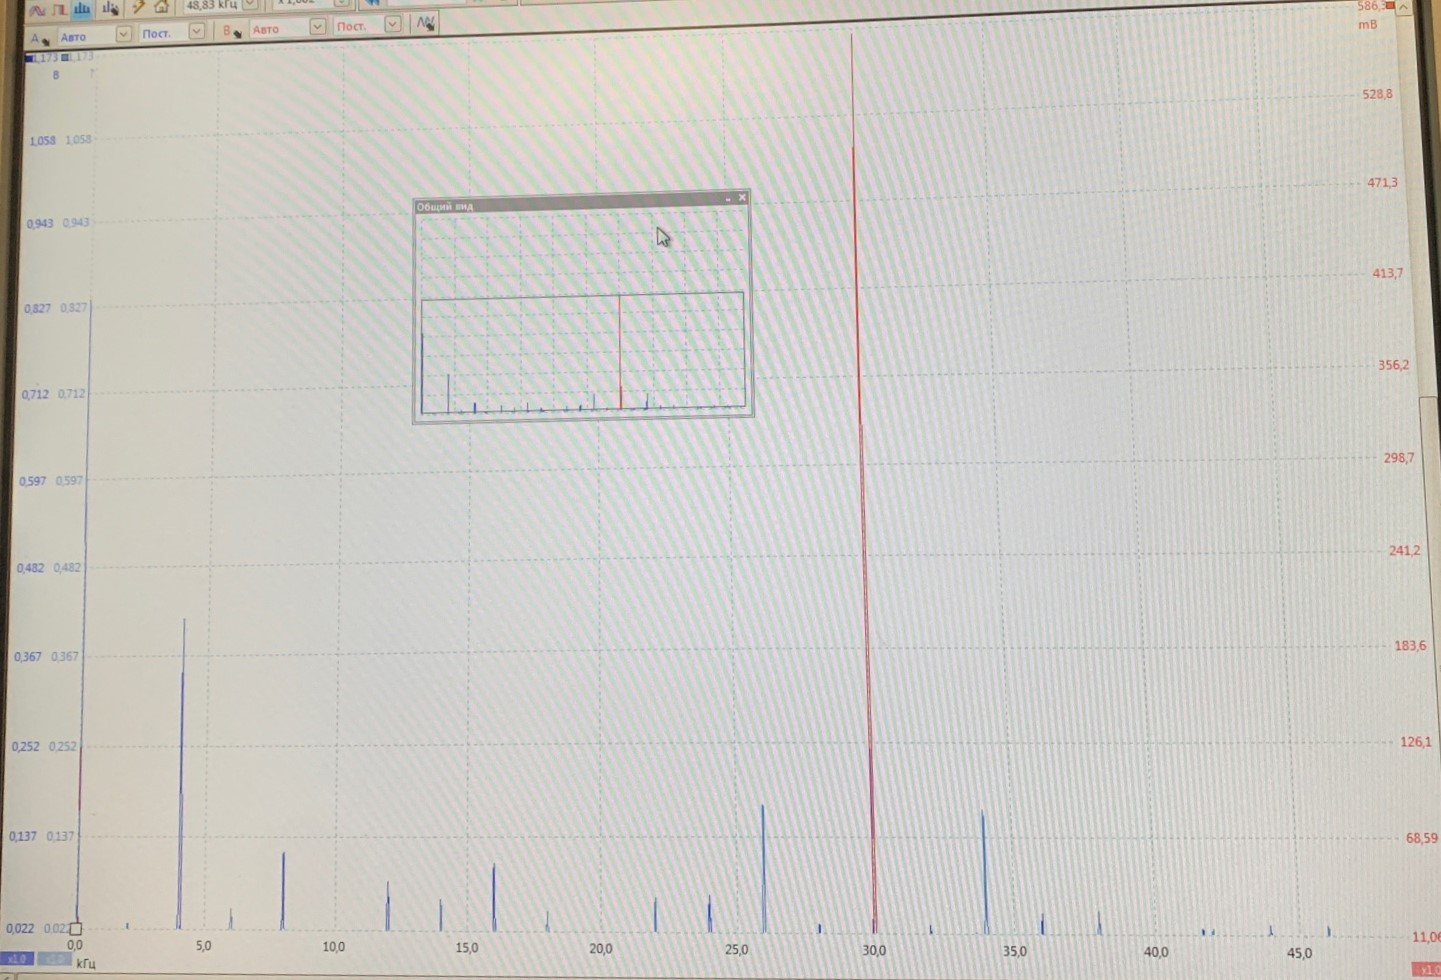
\includegraphics[width=0.45\textwidth]{17.jpg}\\
$f_\text{повт}=$ 2 кГц&$f_\text{повт}=$ 4 кГц\\
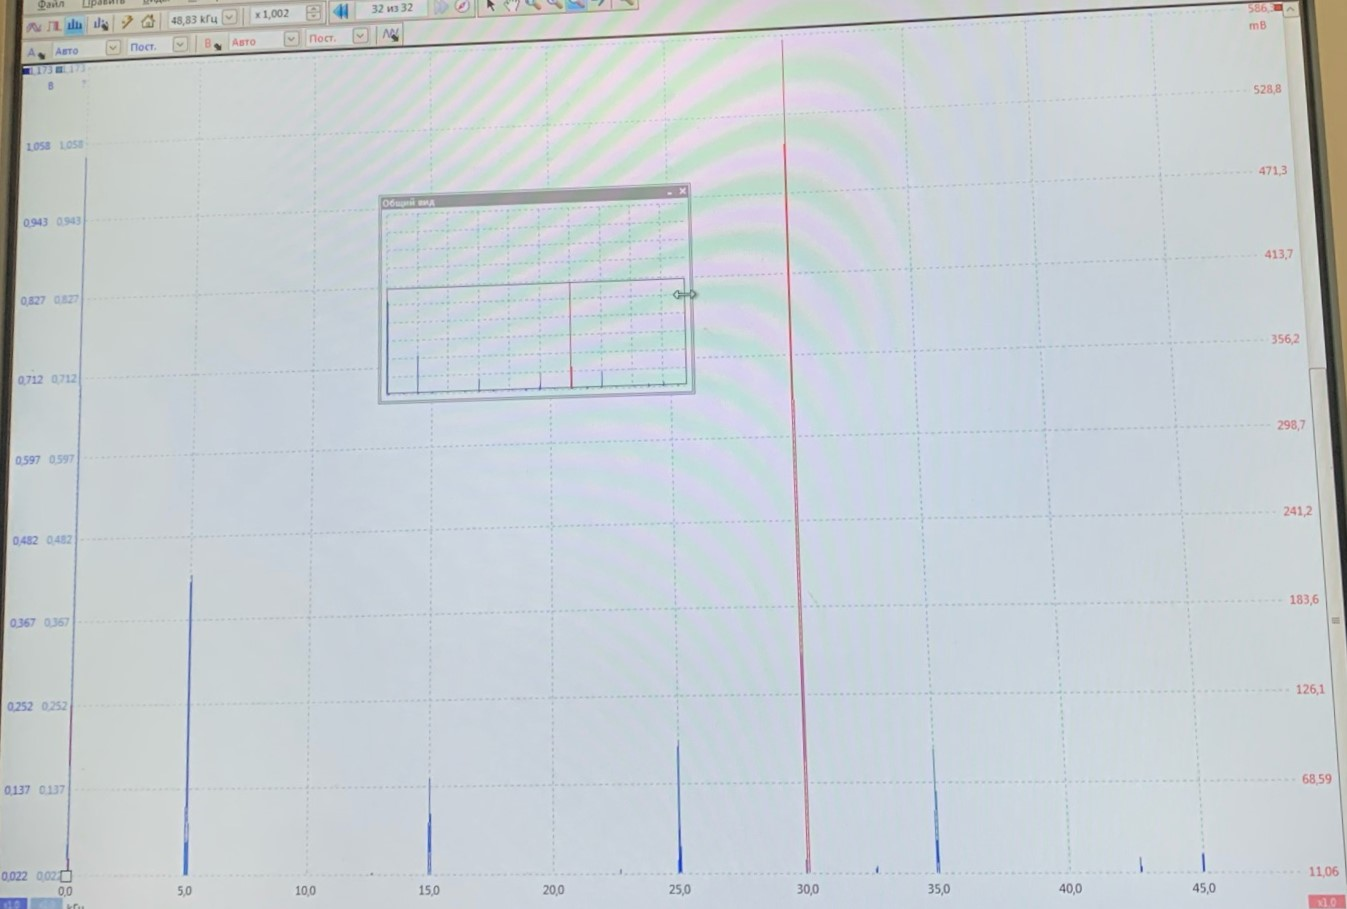
\includegraphics[width=0.45\textwidth]{18.jpg}\\
$f_\text{повт}=$ 5 кГц\\
\end{tabular}
\end{center}

\hfill \break Занесем результаты в таблицу, а также построим график полученной зависимости:

\begin{center}
\begin{tabular}{|c|c|}\hline
$f_\text{повт}$, кГц&$\delta\nu, \text{кГц}$\\\hline
$0.5$&$0.5$\\\hline
$1.0$&$1.0$\\\hline
$2.0$&$2.0$\\\hline
$4.0$&$4.0$\\\hline
$5.0$&$5.0$\\\hline
\end{tabular}\\
\hfill \break \textbf {Таблица 3.} Исследование зависимости $\delta \nu$($f_\text{повт}$)\\
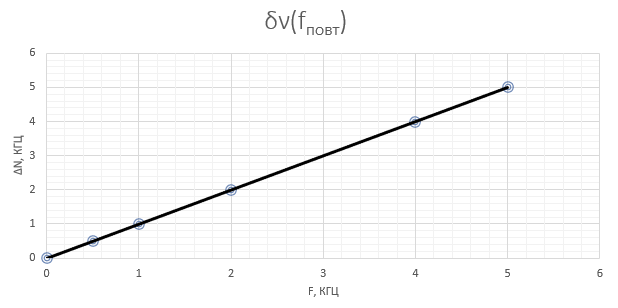
\includegraphics[width=0.95\textwidth]{19.png}\\
График зависимости $\delta \nu$($f_\text{повт}$)~\\
\end{center}

\hfill \break Погрешность результатов определяется погрешностью генератора -- $0.5$ Гц. Таким образом, получаем
$$\frac{\delta\nu, \text{кГц}}{f_\text{повт}} = 1\pm0.1\%,$$
что согласуется с теорией.

\hfill \break Сравнивая спектры прямоугольных импульсов и цугов при $\tau = $ 100 мкс и $f_\text{повт} = $ 1 кГц, можно заметить существенную разницу в положении пиков и величине амплитуды.

\subsection{В. Исследование спектра гармонических сигналов, модулированных по амплитуде}

\hfill \break В этой части исследуем зависимость отношения амплитуд спектральных линий синусоидального сигнала, модулированного низкочастотными гармоническими колебаниями, от коэффициента модуляции, который определяется с помощью осциллографа. Для этого выведем на экран картину амплитудно-модулированного сигнала со следующими параметрами: частота несущей $\nu_{0} = $ 25 кГц, частота модуляции $f_\text{мод} = $ 1 кГц. Меняя двойную амплитуду сигнала от 0.2 до 2 В, измерим для каждого значения максимальную $A_{max}$ и минимальную $A_{min}$ амплитуды сигнала на экране осциллографа и рассчитаем соответствующие значения коэффициента модуляции $m$:

\begin{center}
\begin{tabular}{|c|c|c|c|}\hline
$2A$, В&$A_{max}$, мВ&$A_{min}$, мВ&$m$\\\hline
$0.2$&$548.6$&$450.2$&$0.099$\\\hline
$0.5$&$617.5$&$396.1$&$0.218$\\\hline
$0.8$&$681.4$&$287.8$&$0.406$\\\hline
$1.1$&$754.4$&$223.9$&$0.542$\\\hline
$1.5$&$858.5$&$125.5$&$0.745$\\\hline
\end{tabular}\\
\hfill \break \textbf {Таблица 4.} Исследование зависимости $m$ от $A_{max}$ и $A_{min}$\\
\end{center}

\hfill \break Построим график отношения $a_\text{бок}/a_\text{осн}$ в зависимости от $m$ и определим его угловой коэффициент наклона.

\begin{center}
\begin{tabular}{|c|c|c|c|}\hline
$a_\text{бок}$, мВ&$a_\text{осн}$, мВ&$k = a_\text{бок}/a_\text{осн}$&$m$\\\hline
$16$&$322$&$0.05$&$0.10$\\\hline
$47$&$322$&$0.15$&$0.30$\\\hline
$75$&$322$&$0.23$&$0.50$\\\hline
$107$&$322$&$0.33$&$0.70$\\\hline
$139$&$322$&$0.43$&$0.90$\\\hline
\end{tabular}\\
\hfill \break \textbf {Таблица 5.} Исследование зависимости $a_\text{бок}/a_\text{осн}$ от $m$\\
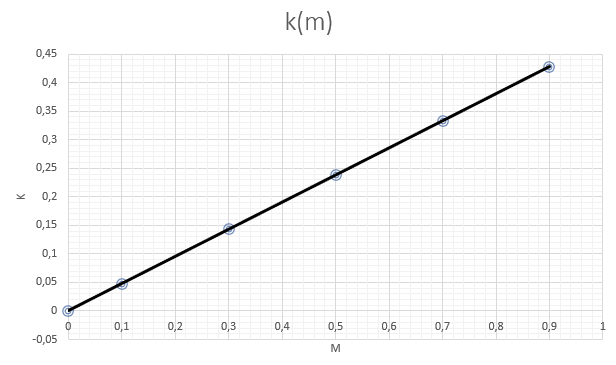
\includegraphics[width=0.95\textwidth]{21.png}\\
График зависимости $a_\text{бок}/a_\text{осн}$ ($m$)~\\
\end{center}

\hfill \break Из графика получаем коэффициент наклона, равный $0.476\pm 0.015$. По формуле $a_\text{бок}=a_\text{осн}m/2$, откуда $k_\text{теор} = $ 0.5, что согласуется с экспериментальным значением, полученным в данной работе. 

\section{Вывод}

\hfill \break В данной работе мы провели исследование нескольких типов периодических сигналов: исследовали их разложение в гармонический спектр, получили картины спектров, а также проверили справедливость нескольких соотношений. Так, мы убедились в верности соотношения неопределенностей, исследовали зависимость расстояния между соседними спектральными компонентами от частоты повторения цугов. В заключительной части работы коэффициенты, полученные в результате исследования зависимости отношения амплитуд спектральных линий синусоидального сигнала, модулированного низкочастотными гармоническими колебаниями, от коэффициента модуляции в пределах погрешности совпали с рассчитанными теоретически.

\end{document}